\documentclass[11pt, a4paper]{article}
\usepackage{rminterim}
\begin{document}
% Your project title etc goes here
\title{\textsc{\huge 5M02 MICROELECTRONIC CIRCUITS }\\ {\Large Laboratory 1}}
\author{Patrick Owens \\ 16317356}
%\address{Interim Report}

\date{\today}



\maketitle

\begin{center}
\begin{minipage}[t]{0.75\linewidth}
\textit{
I have read and I understand the plagiarism provisions in the General Regulations of the University Calendar for the current year, found at \myhref{http://www.tcd.ie/calendar}{http://www.tcd.ie/calendar}. \\
I have also completed the Online Tutorial on avoiding plagiarism ‘Ready Steady Write’, located at 
\myhref{http://tcd-ie.libguides.com/plagiarism/ready-steady-write}{http://tcd-ie.libguides.com/plagiarism/ready-steady-write}.}
\end{minipage}
\end{center}

\newpage





\section{Transistor Characteristics}
\subsection{Drain Current-Drain Voltage} \label{sec:circ1}

The circuit in figure\ref{fig:circuit1} was constructed to characterise transistor U1. In this experiment the gate-source voltage, $V_{GS}$ is held constant and the drain-source voltage $V_{DS}$ is varied from $0 - 5V$, a current probe is attached to the drain terminal of transistor U1 in order to monitor the drain current as $V_{DS}$ is varied.

\begin{wrapfigure}{r}{0.5\textwidth}
  \centering
    \caption{Circuit to characterise transistor U1.}
    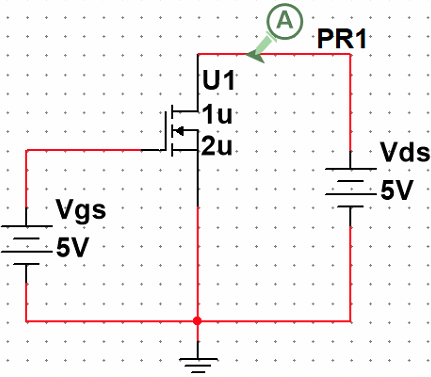
\includegraphics[width=0.48\textwidth]{report/img/question_2/circ1.png}
    \label{fig:circuit1}
\end{wrapfigure}




The current-voltage characteristic of the circuit produced from sweeping the value of $V_{DS}$ from 0V to 5V can be seen in figure \ref{fig:graph1}. 

As can be seen in figure \ref{fig:graph1} the saturation value of the drain current $I_{D_{Sat}} = 320 \mu A$ and the saturation value of the drain-source voltage $V_{DS_{Sat}} = 4.797V$.

The values for $I_{D_{Sat}}$ and $V_{DS_{Sat}}$ from figure \ref{fig:graph1} can be verified using equations \ref{eq:1} and \ref{eq:pt2}.
\begin{equation}
  \label{eq:1}
  I_{D_{Sat}} = \frac{1}{2}\beta_{n}\frac{W}{L}\bigg(V_{GS} - V_T\bigg)
\end{equation}
\begin{equation}
    V_{DS_{Sat}} = V_{GS} - V_T
    \label{eq:pt2}
\end{equation}
In equation \ref{eq:1} the conductance parameter of the transistor is $\beta_n = 20 \mu A/V$ , the channel width 
is $W = 2\mu M$, the channel length is $L = 1 \mu M$, the gate-source Voltage is $V_{GS} = 5V$
and the threshold voltage is $V_T = 1V$. Using these values in equations \ref{eq:1} and \ref{eq:pt2} we can verify that the value of $I_{D_{Sat}}$ $V_{DS_{Sat}}$ from figure \ref{fig:graph1}:
\begin{gather}
    I_{D_{Sat}} = \frac{1}{2}20 \mu AV^{-1}\frac{2\mu M}{1 \mu M}\bigg(5V - 1V\bigg) = 322 \mu A \\
    V_{DS_{Sat}} = 5V - 1V = 4V 
\end{gather}    

\begin{figure}
  \centering
  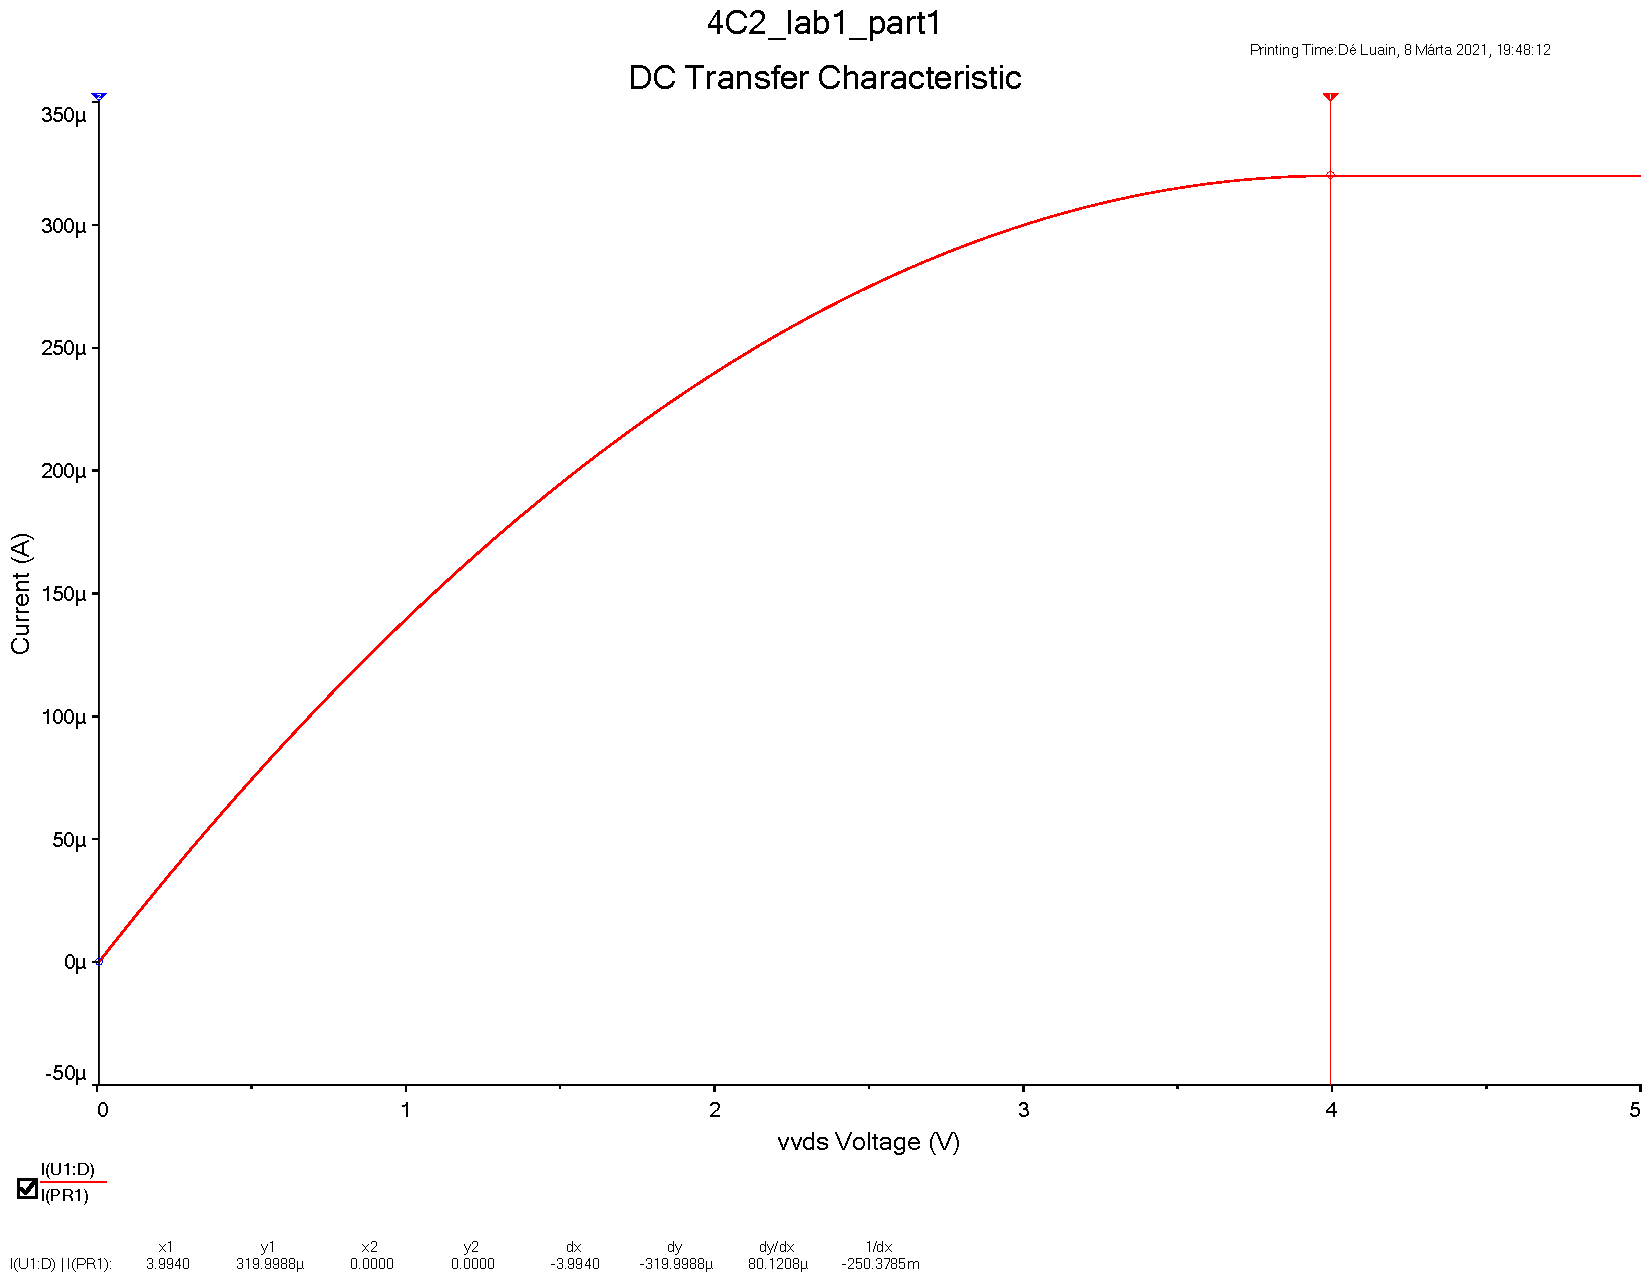
\includegraphics[width=\textwidth]{report/img/question_2/g1.pdf}
  \caption{\centering Current-voltage plot for transistor U1, showing the value for $I_{D_{Sat}} = 320 \mu A$ and $V_{DS} = 4V$}
    \label{fig:graph1}
\end{figure}

\newpage
\subsection{Comparison of Transistor Characteristics}

\begin{wrapfigure}{r}{0.5\textwidth}
  \centering
    \caption{Circuit constructed to compare the characteristics of transistors U1 and U2.}
    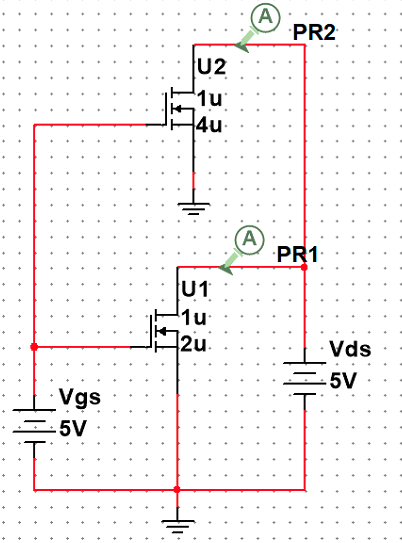
\includegraphics[width=0.45\textwidth]{question_2/circ2.png}
    \label{fig:circuit2}
\end{wrapfigure}


The circuit in figure \ref{fig:circuit1} has been modified by adding another transistor U2 in parallel to transistor U1, a current probe is also attached to the drain terminal of transistor U2. Comparison of the characteristics of the transistors in this circuit can be done following the same process as in section \ref{sec:circ1}. 

The results of the characterisation can be seen in figure \ref{fig:graph2}.

It can be seen in figure \ref{fig:graph2} that the plot of $V_{DS}$ versus $I_D$ for transistor U1 remains unchanged from figure \ref{fig:graph1}, with the same values for $I_{D_{Sat}}$ and $V_{DS_{Sat}}$.

Transistor U2 has a drain current saturation value $I_{D_{Sat}} = 640 \mu A$ and a drain-source voltage saturation value $V_{DS} = 4V$.\\ These values are to be expected as the channel width of transistor U2 is double that of transistor U1 and as such it's value for $I_{D_{Sat}}$ is accordingly double. The values of $I_{D_{Sat}}$ and $V_{DS_{Sat}}$ for transistor U2 can be verified using the equations \ref{eq:1} and \ref{eq:pt2} from section \ref{sec:circ1}.

\begin{gather}
    I_{D_{Sat}} = \frac{1}{2}20 \mu AV^{-1}\frac{4\mu M}{1 \mu M}\bigg(5V - 1V\bigg) = 644 \mu A \\
    V_{DS} = 5V - 1V = 4V 
\end{gather}

\begin{figure}
  \centering
  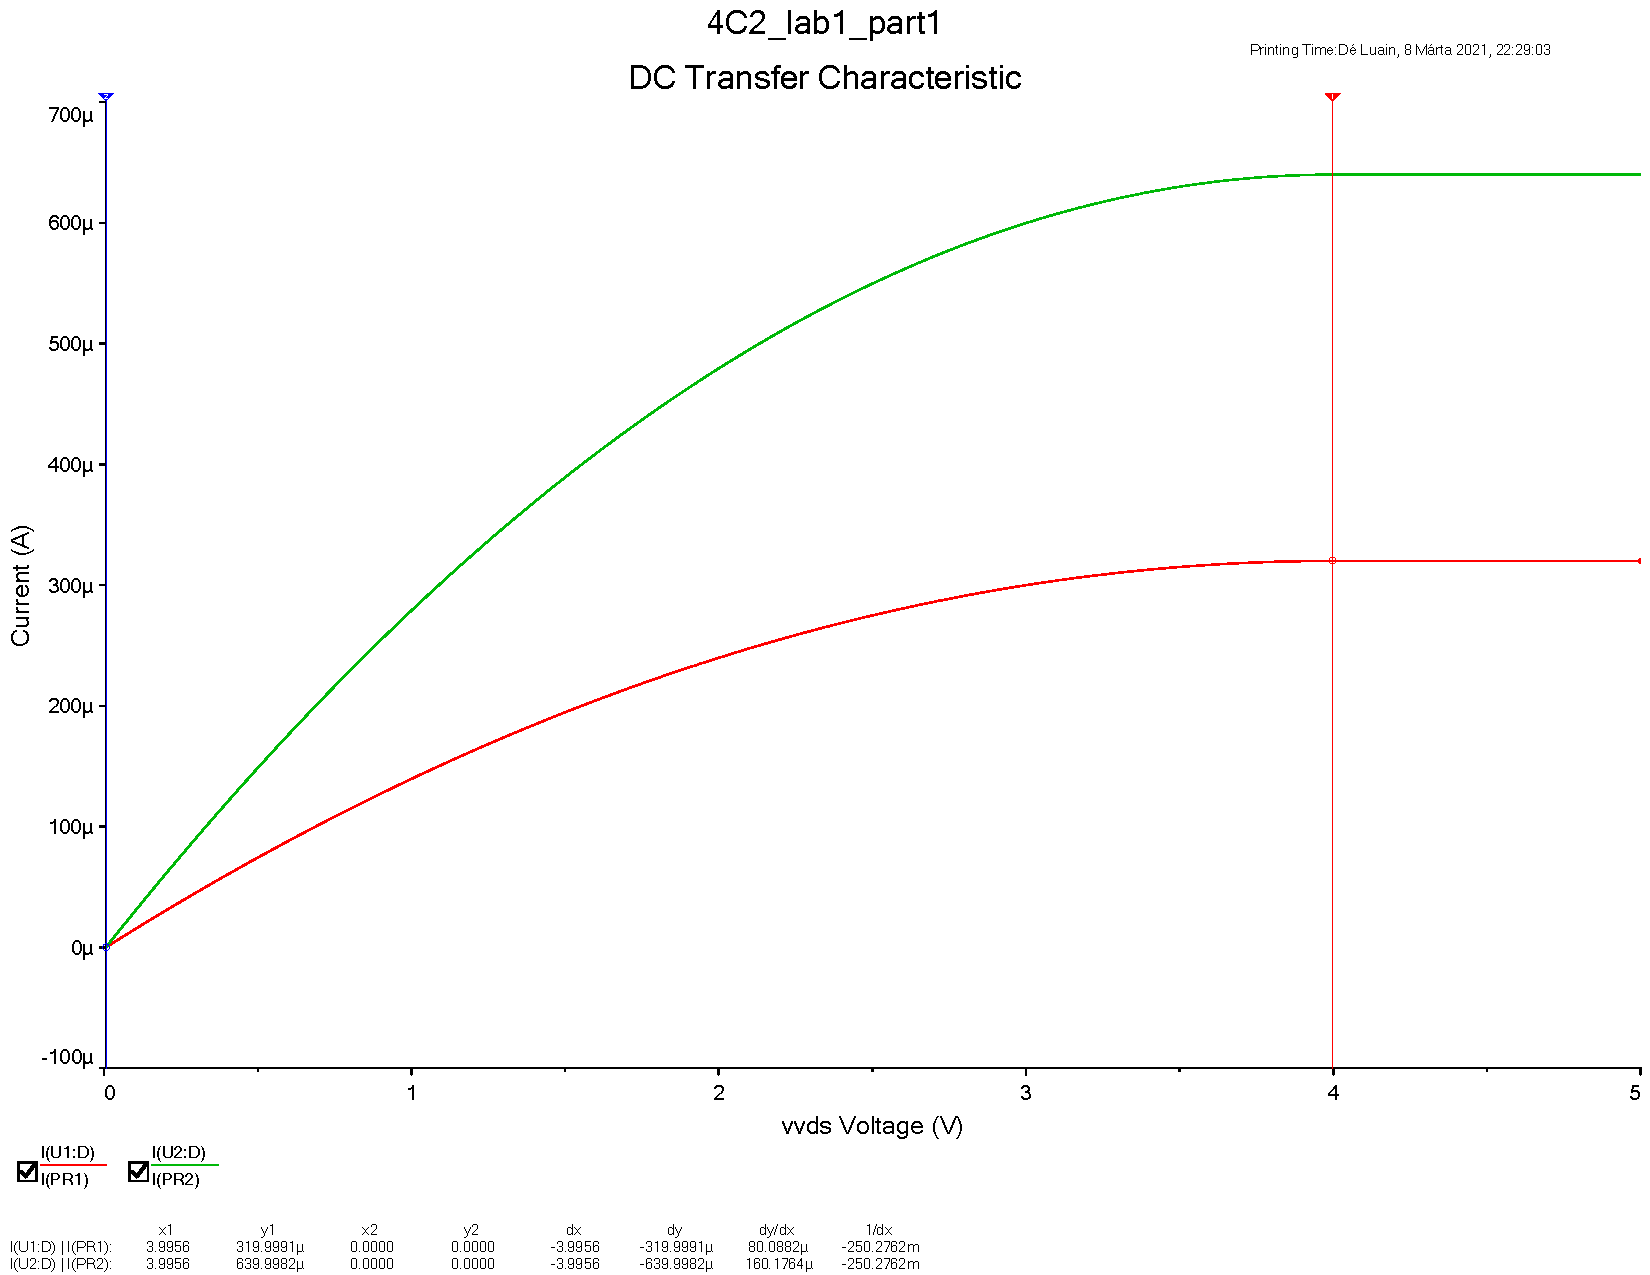
\includegraphics[width=\textwidth]{question_2/g2.pdf}
  \caption{\centering Current-voltage plot for transistors U1 and U2, showing the values for $I_{D_{Sat}} = 320 \mu A$ and $V_{DS} = 4V$for transistor U1, and $I_{D_{Sat}} = 640 \mu A$ and $V_{DS_{Sat}} = 4V$ for transistor U2.}
    \label{fig:graph2}
\end{figure}

\FloatBarrier
\subsection{Channel Length Modulation}
In the circuit in figure \ref{fig:circuit2}, changing transistor U2 so that it's with is $W = 2 \mu M$, adding a channel length modulation parameter, $\lambda = 0.02 V^{-1}$ and re-running the simulation will produce the current-voltage graph in figure \ref{fig:graph3}.

With transistors U1 and U2 having identical widths, the effect of channel length modulation ($\lambda$) on transistor U2 can be clearly seen.

As the voltage $V_{DS_{Sat}}$ is increased channel length modulation will cause the channel length to be reduced, this has the effect of increasing the drain current $I_ {D}$, as shown in figure \ref{fig:graph3}.

The impact of channel length modulation is most apparent in the saturation region. Where the current $I_{D}$ will now increase linearly with $V_{DS}$, the rate of increase is determined by the empirical channel length modulation parameter $\lambda = 0.02 V^{-1}$.

As the largest impact of channel length modulation occurs in the saturation region equation \ref{eq:1} must be modified to account for its effect. Equation \ref{eq:1.2.1} can be used to describe the drain current ($I_{D}$) in the saturation region accounting its impact.

\begin{equation}
    I_{D_{Sat}} = \frac{1}{2}\beta_{n}\frac{W}{L}\bigg(V_{GS} - V_T\bigg) \times \bigg(1 + \lambda V_{DS}\bigg)
    \label{eq:1.2.1}
\end{equation}




\begin{figure}
  \centering
  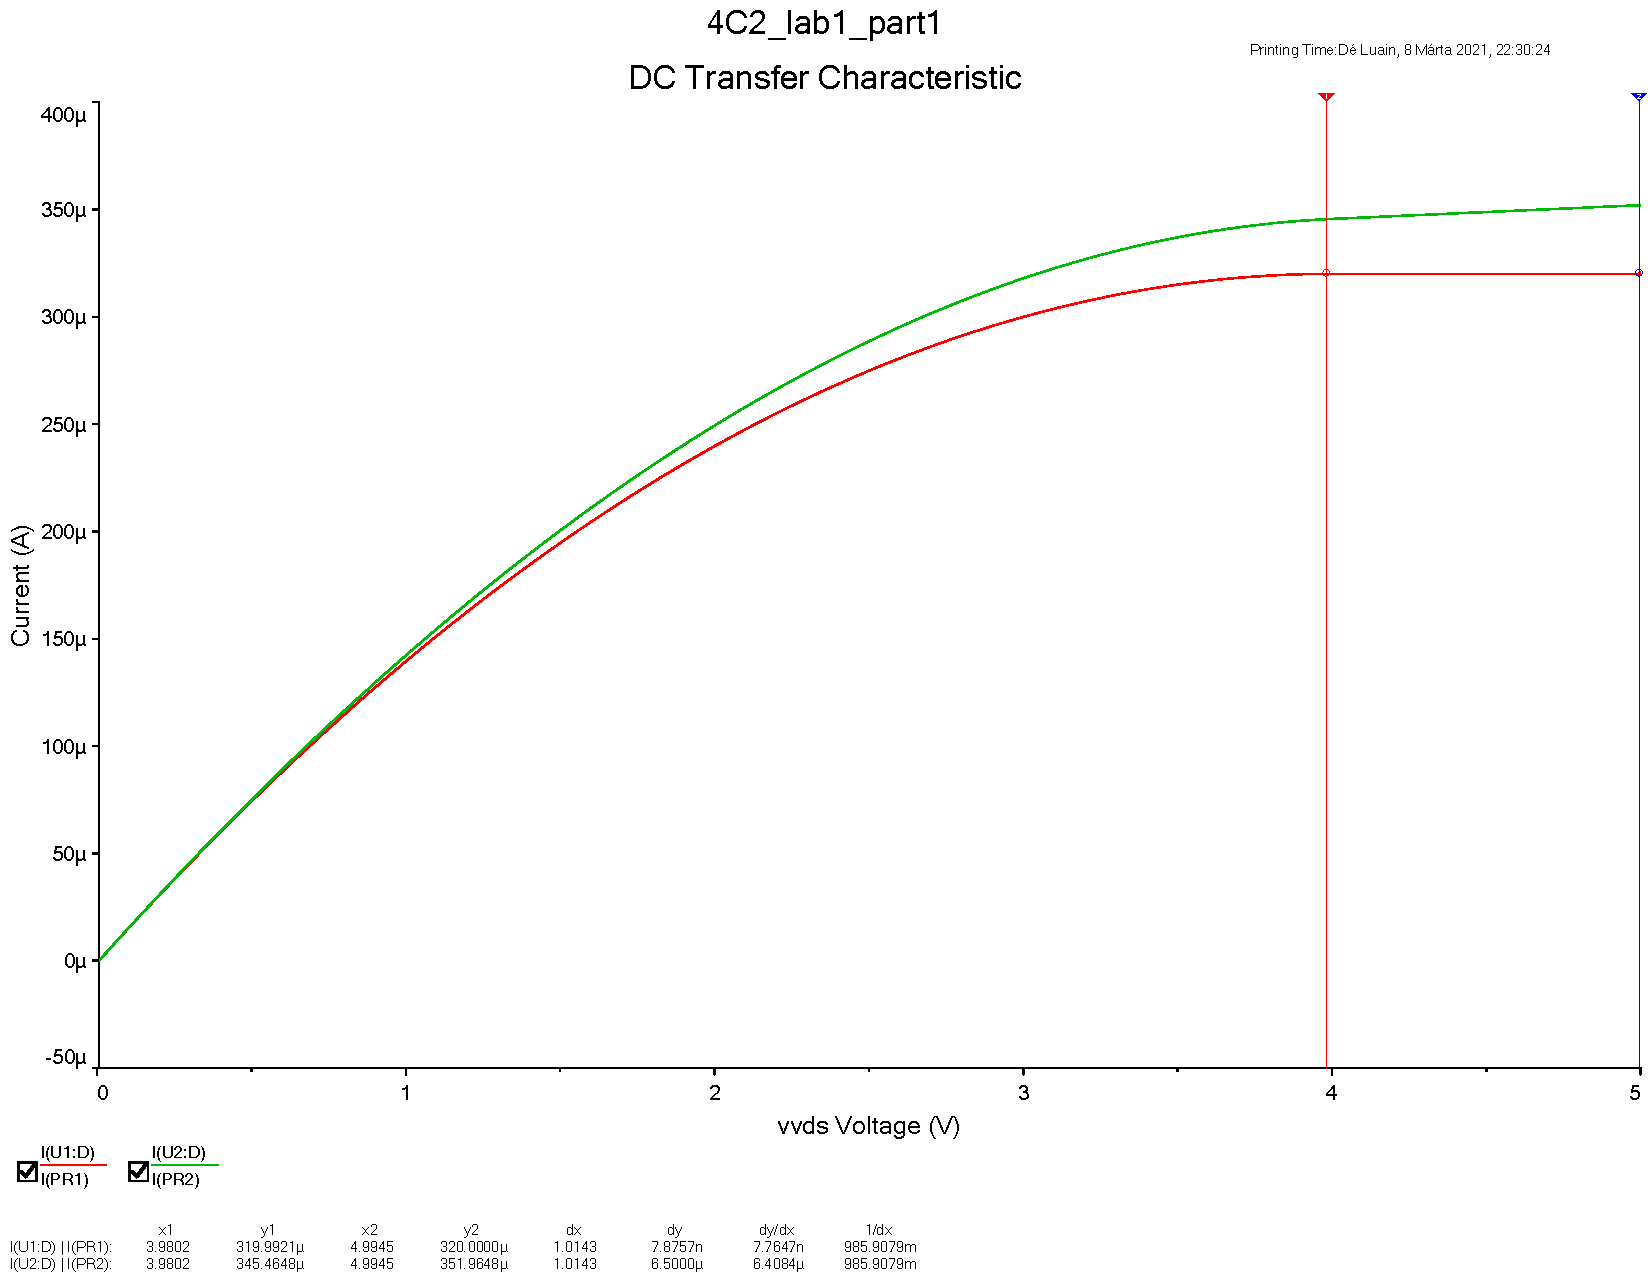
\includegraphics[width=\textwidth]{question_2/g3.pdf}
  \caption{\centering Current-voltage plot for transistors U1 and U2, showing the effect of channel length modulation on transistor U2. $I_{D_{Sat}}$ increases from $345 \mu A$ at $V_{DS} = 4V$ to $352 \mu A$ at $V_{DS} = 5V$.}
    \label{fig:graph3}
\end{figure}
\FloatBarrier

\newpage
\section{Resistor Load Inverters}


\subsection{R1 = 25k$\Omega$}
\subsubsection{Output Characteristic}

\begin{wrapfigure}{R}{0.5\textwidth}
  \centering
    \caption{Circuit constructed to measure the output characteristic of transistor U1.}
    \label{fig:circuit3}
    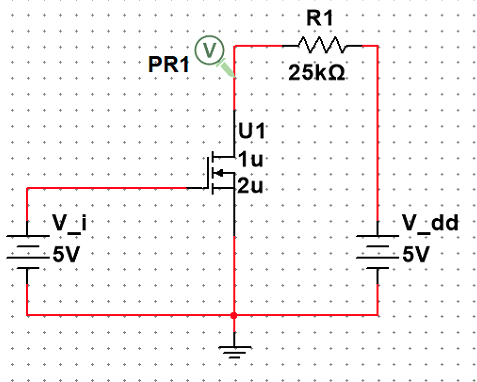
\includegraphics[width=0.45\textwidth]{question_3/circuit3.png}
\end{wrapfigure}

The circuit in figure \ref{fig:circuit3} was constructed to measure the transfer characteristic of transistor U1 for various values of R.

A plot of the transfer characteristic for this circuit configuration can be produced by sweeping the input voltage ($V_i$) from 0V to 5V and measuring the output voltage of transistor U1 using probe PR1.

\begin{figure}
  \centering
  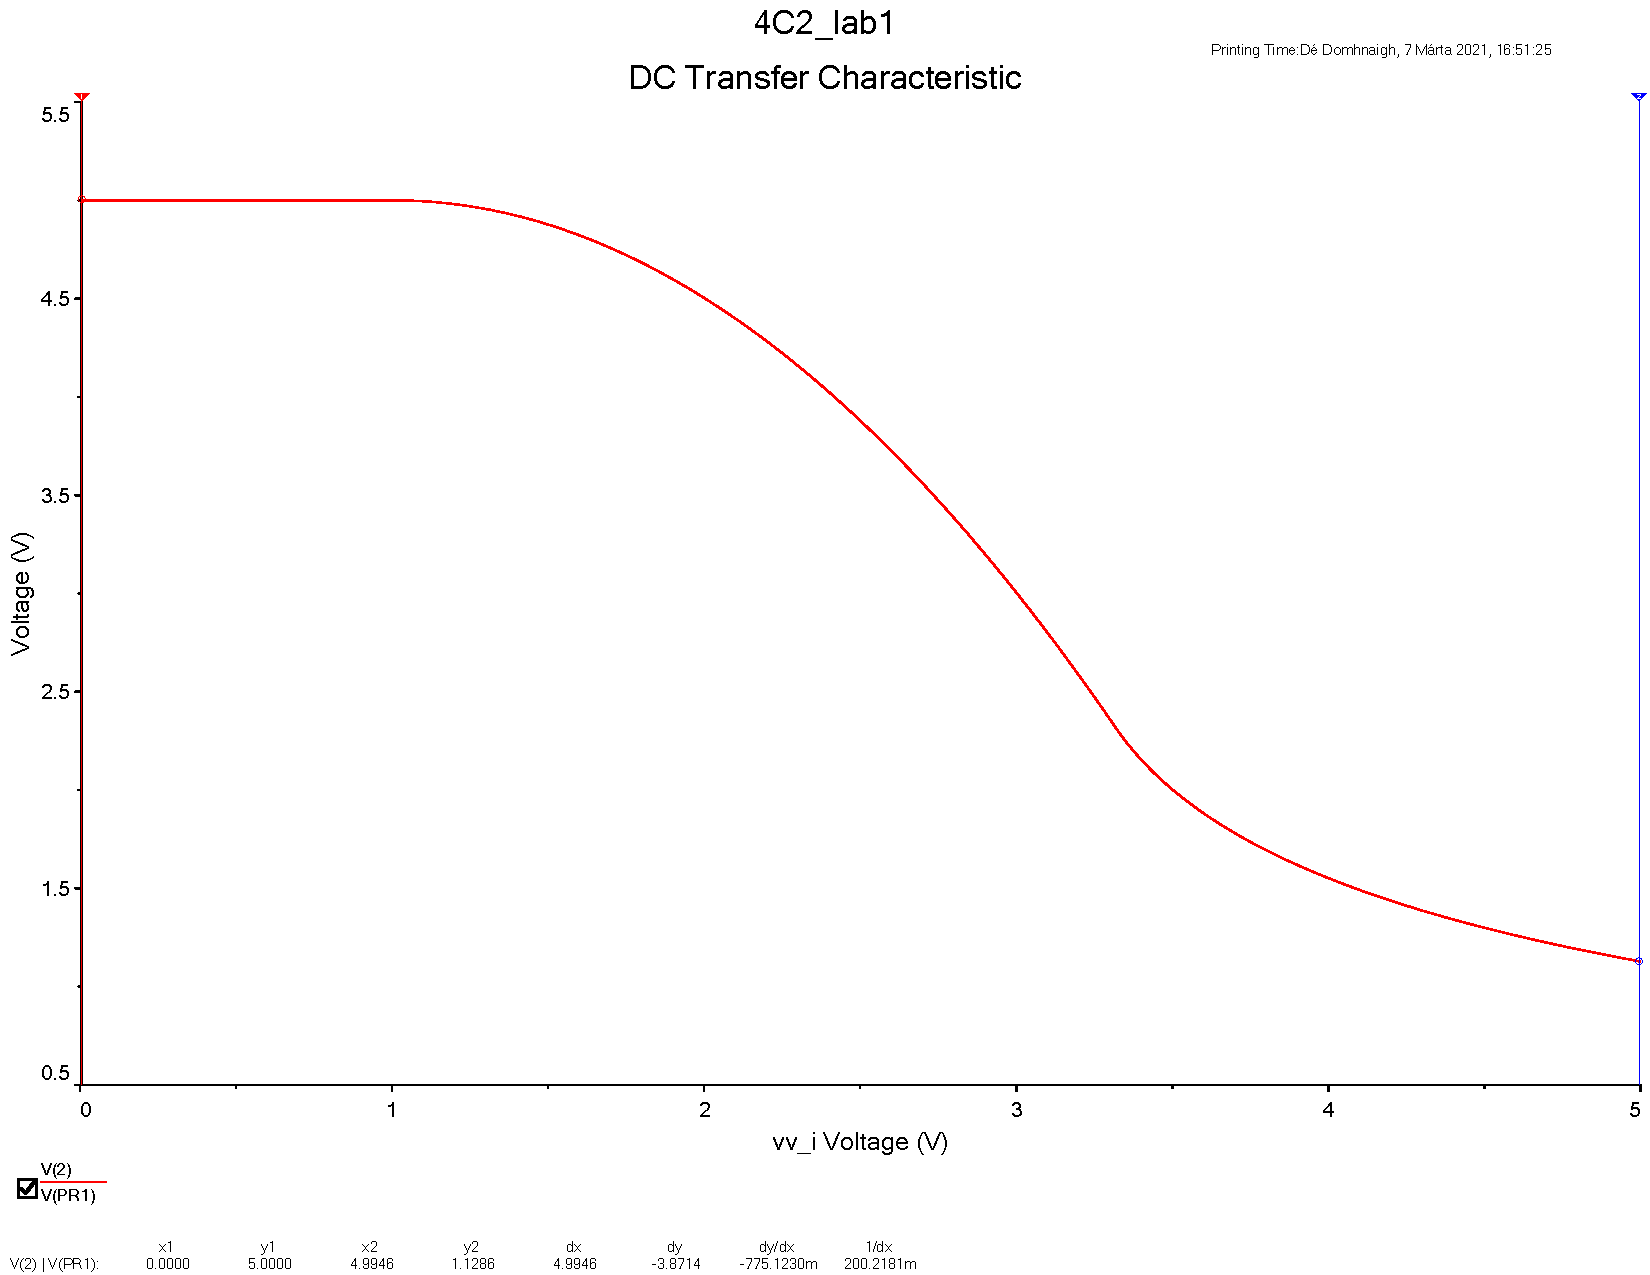
\includegraphics[width=\textwidth]{question_3/25k_ohm.pdf}
  \caption{\centering Output characteristic of the circuit in figure \ref{fig:circuit3} when R = $25k \Omega$, showing a value of $V_O = 1.129V$ when $V_i = V_{DD}$.}
    \label{fig:graph4}
\end{figure}

For $R = 25k\Omega$ the transfer characteristic of the circuit can be seen in figure \ref{fig:graph4}.\\
When $V_i$ < $V_T$;\\ $V_O = V_{DD} = 5V$, this is confirmed in figure \ref{fig:graph4}.

When $V_i = V_{DD}$;\\ $V_O$ can be calculated using equation \ref{eq:2.1}:
\\~\\
\begin{equation}
  V_O = V_{DD} - V_T + \frac{1}{\beta R} \pm \sqrt{\bigg(V_{DD} - V_T + \frac{1}{\beta R} \bigg)^2 - \frac{2V_{DD}}{\beta R}}
  \label{eq:2.1}
\end{equation}

Where $V_O  $ is the output voltage, $V_{DD} = 5V$, the threshold voltage is $V_T = 1V$, resistance is 
$R = 25\Omega$, and the conductance parameter is $\beta = 4\mathrm{e}{-5}$. $\beta$ can be calculated using equation \ref{eq:2.1.1} and the following values $\mu_n C_{ox} = 20 \mu A V^{-1}$ and $\frac{W}{L} = 2$ :
\begin{equation}
    \beta = \mu_n C_{ox} \times \frac{W}{L}
    \label{eq:2.1.1}
\end{equation}
 \par
Using the above values with equation \ref{eq:2.1} will produce the value of $V_O = 1.127V$ which matches the value of $V_O$ in figure \ref{fig:graph4}.

\FloatBarrier
\subsubsection{$V_{OH}$, $V_{IL}$, $V_{OL}$, $V_{IH}$ calculation}

\begin{figure}
  \centering
  \begin{minipage}{0.7\textwidth}
      \centering
      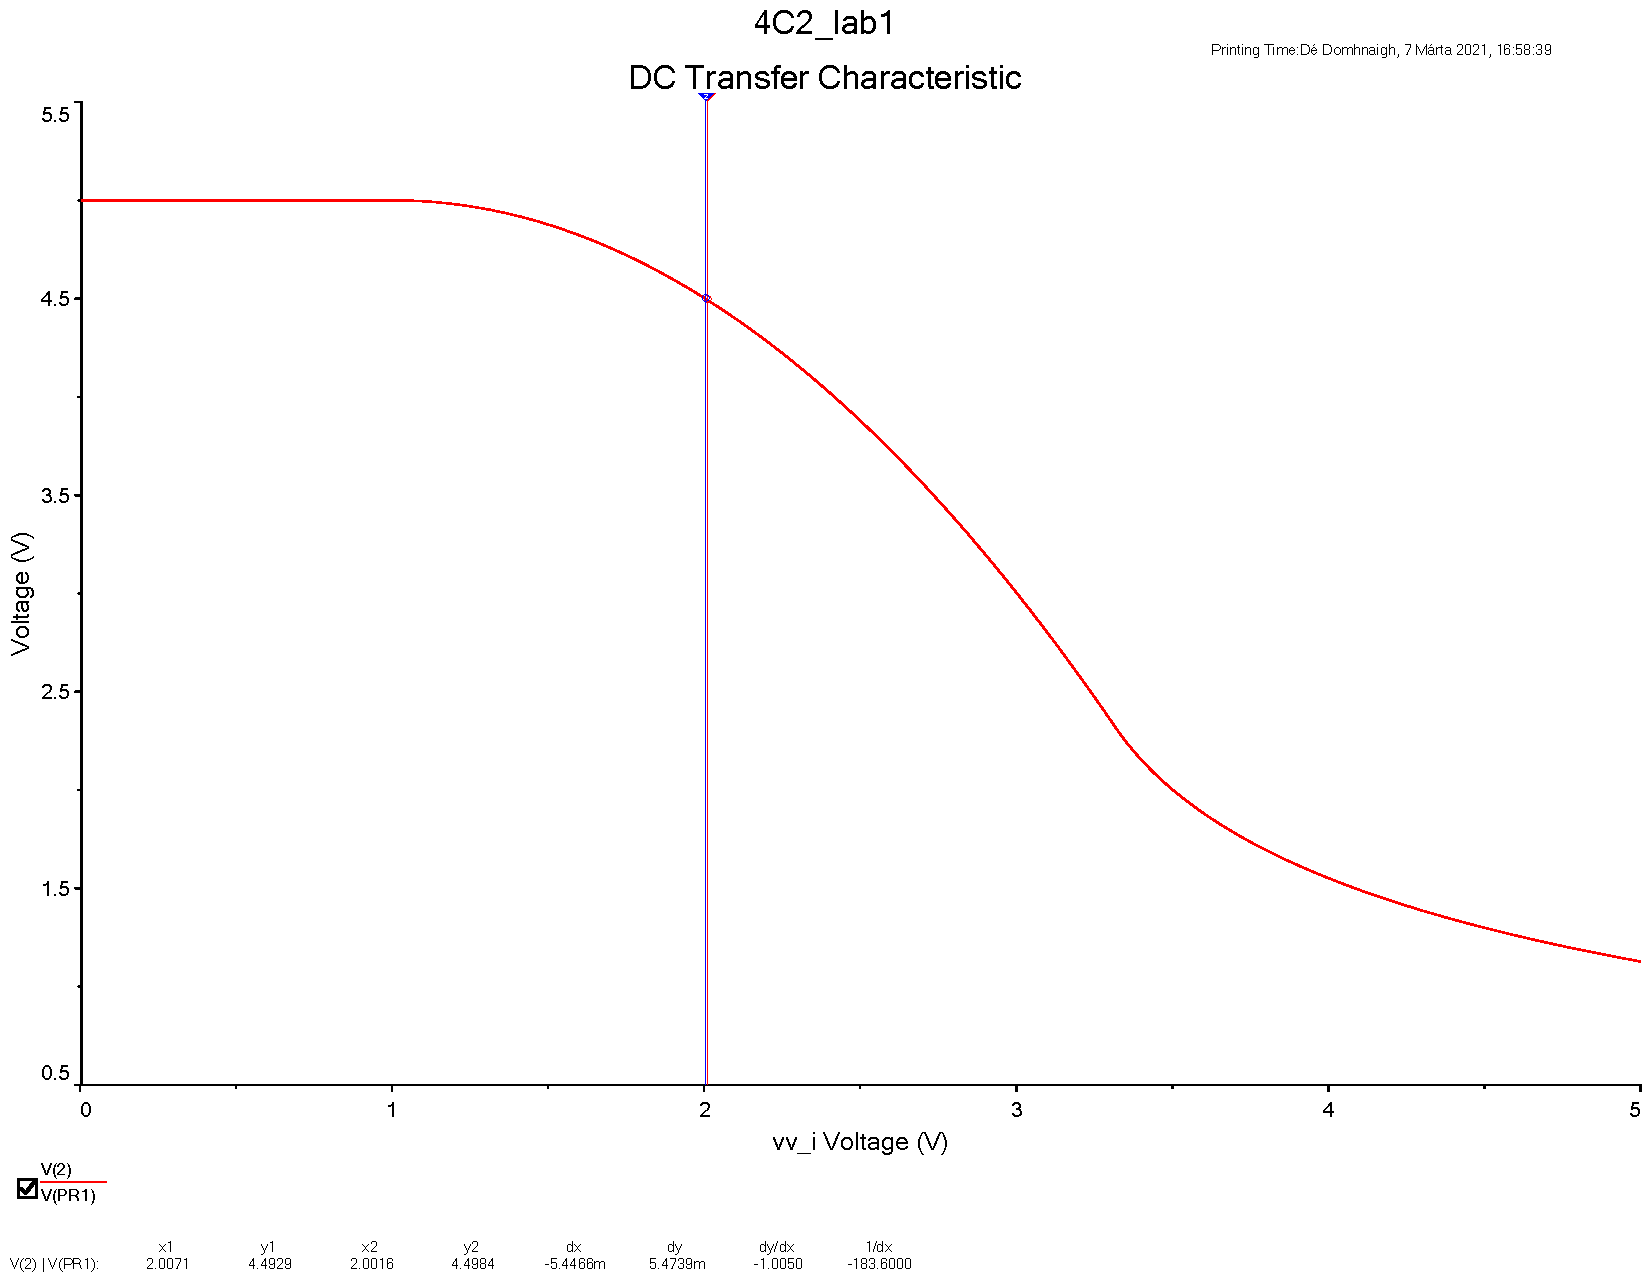
\includegraphics[width=\textwidth]{question_3/25k_ohm_voh_vil} % first figure itself      
  \end{minipage}\vfill
  \begin{minipage}{0.7\textwidth}
      \centering
      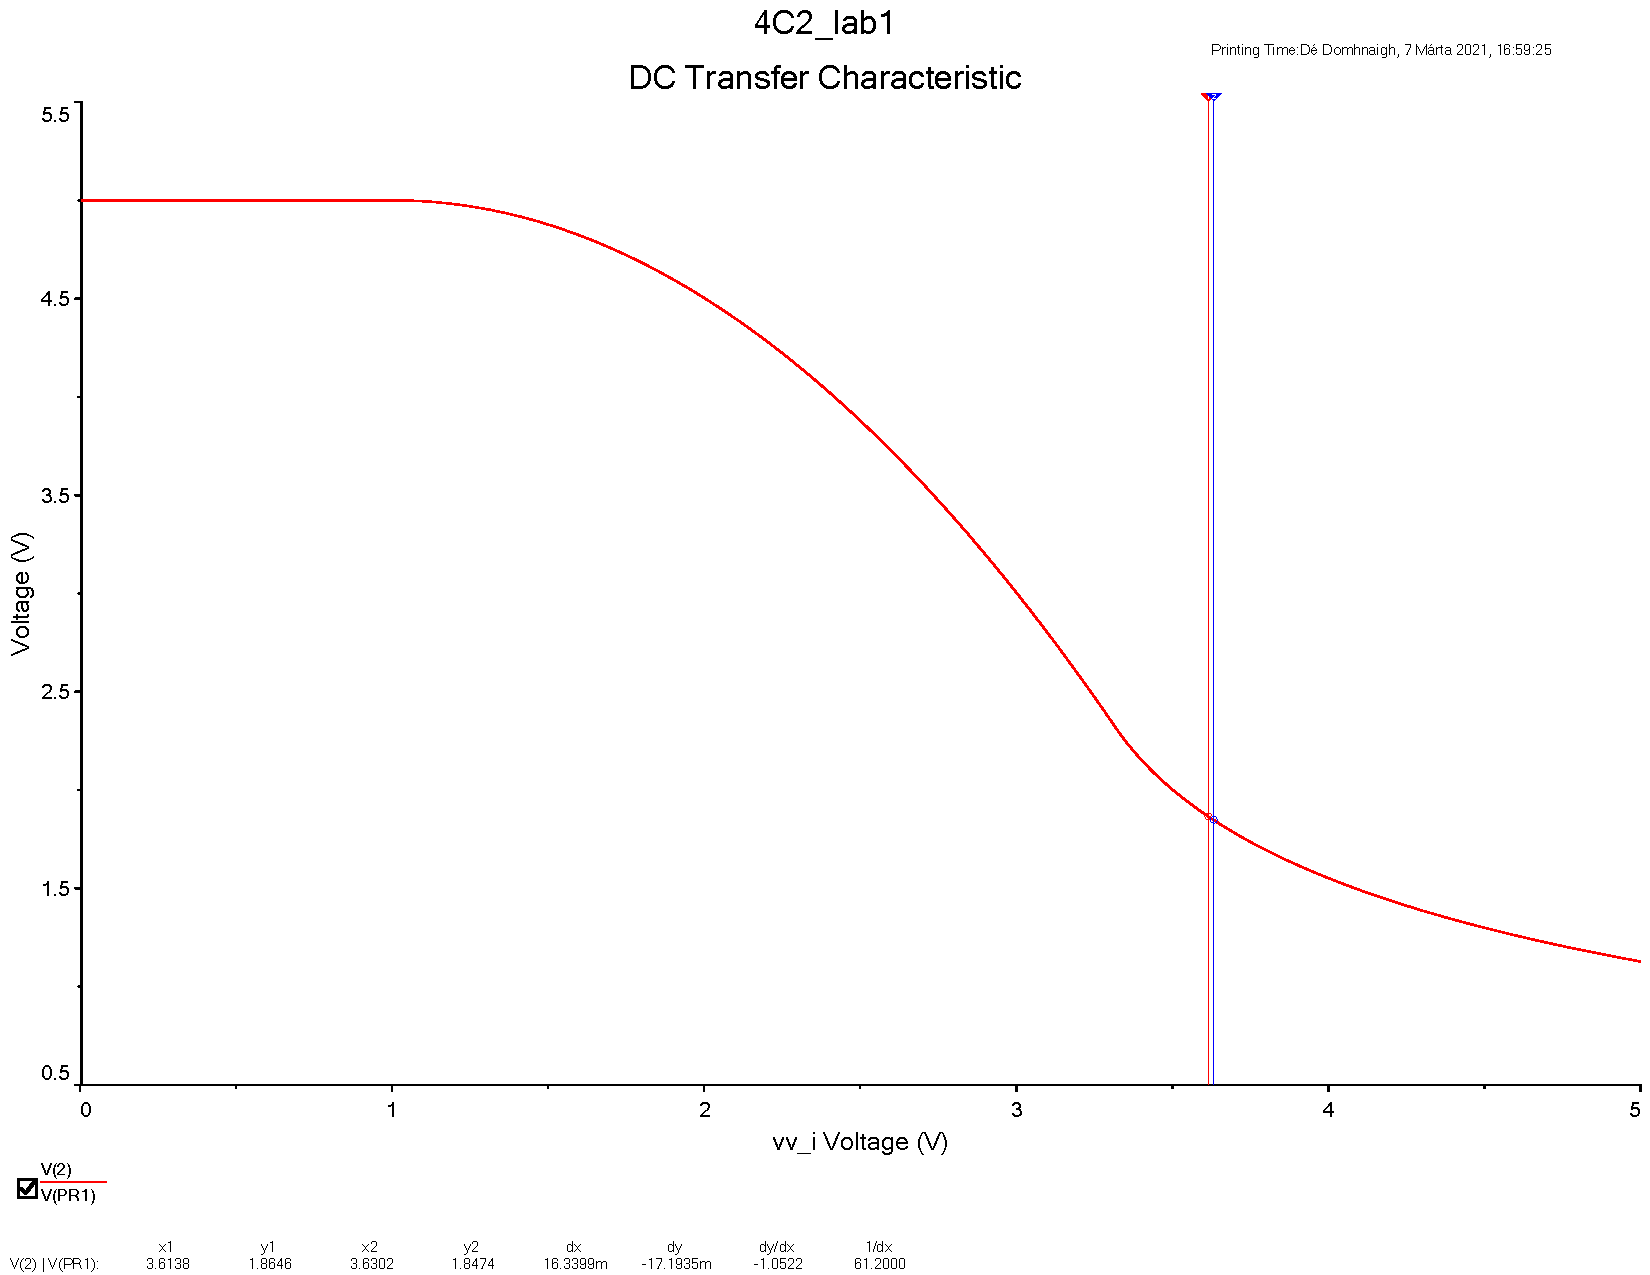
\includegraphics[width=\textwidth]{question_3/25k_ohm_vol_vih} % second figure itself      
  \end{minipage}
  \caption{\centering Plots showing $V_{OH} = 4.5V$ and $V_{IL} = 2V$ (top), and $V_{OL} = 1.825V$ and
   $V_{IH} = 3.638$ (bottom), for $R = 25k\Omega$}  
   \label{fig:8}
\end{figure}

From figure \ref{fig:8} we can see the values of voltage output-high, $V_{OH} = 4.5V$, voltage input-low $V_{IL} = 2V$, voltage output-low $V_{OL} = 1.825V$, and voltage input-high $V_{IH} = 3.638$ for the circuit in figure \ref{fig:circuit3} all closely match the expected values of these quantities which have been calculated below.



    

\begin{gather}    
V_{OH} = 5 - \frac{1}{2\Beta R}\label{eq:2.1.2.1}\\
V_{OH} = 5 - \frac{1}{2} \times 1 = 4.5V\\
V_{IL} = V_T + \frac{1}{\Beta R}\label{eq:2.1.2.2}\\
V_{IL} = 1 + 1 = 2V \\
V_{OL} = \sqrt{\frac{2}{3} \times \frac{V_{DD}}{\Beta R}}\label{eq:2.1.2.3}\\
V_{OL} = \sqrt{\frac{2}{3} \times 5 \times 1} = 1.825V\\
V_{IH} = V_T + \sqrt{\frac{8}{3} \times \frac{V_{DD}}{\Beta R}}\label{eq:test}\label{eq:2.1.2.4}\\
V_{IH} = 1 + \sqrt{\frac{8}{3} \times 5 \times 1} - 1 = 3.65V
\end{gather}

Channel length modulation results in the reduction of the effective channel length as a result of $V_{DS}$ increasing. 
Since $\beta \propto \frac{W}{L}$ and $-L \propto \lambda$ increasing $\lambda$ will lead to an increase in $\beta$. Increasing $\beta$ causes the value of $V_{OL}$ to be reduced, and the voltage transfer characteristic of the transistor to move towards ideality.

\FloatBarrier
\subsection{R1 = 100k$\Omega$}
\subsubsection{Output Characteristic}

\begin{figure}[h]
  \centering
  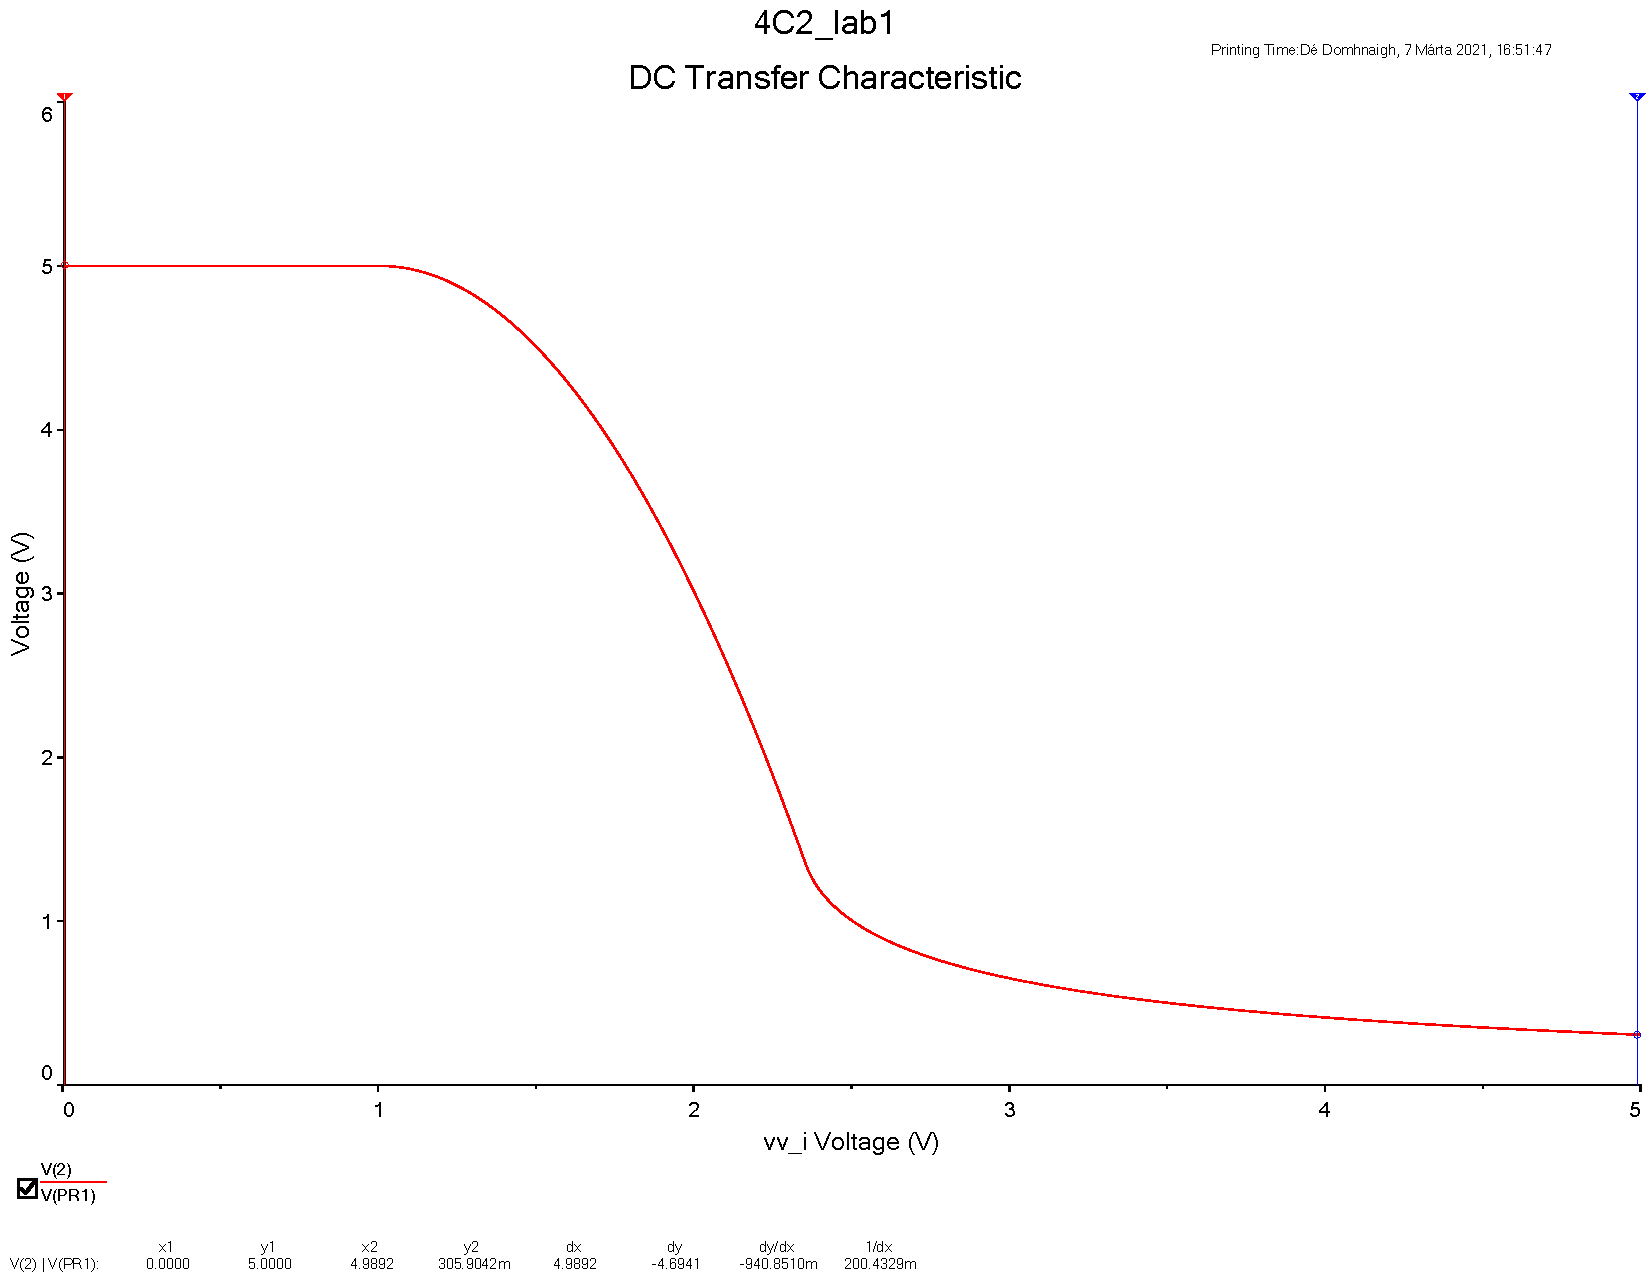
\includegraphics[width=\textwidth]{question_3/100k_ohm.pdf}
  \caption{\centering Output characteristic of the circuit from figure \ref{fig:circuit3} when R = $100k \Omega$, showing a value of $V_o = 0.306V$ when $V_i = V_{DD}$.}
    \label{fig:9}
\end{figure}


When $V_i$ < $V_T$, $V_o = {V_{DD}} = 5V$ as can be seen in figure \ref{fig:9}.

Using equation \ref{eq:2.1} and the following values, $V_{DD} = 5V$, $V_T = 1V$, $R = 100k\Omega$ and
$\beta = 4\mathrm{e}{-5} AV^{-1}$, to calculate $V_o$, when $V_i = V_{DD}$:
\begin{equation}
  0.305 = 5 - 1 + \frac{1}{100 \times 4\mathrm{e}{-5} } \pm \sqrt{\bigg(5V - 1V + \frac{1}{100k \Omega \times 4\mathrm{e}{-5}} \bigg)^2 - \frac{2 \times 5}{100 \times 4\mathrm{e}{-5}}}
  \label{eq:2}
\end{equation}
The value of $V_o = 0.305V$ matches the value of $V_o$ from figure \ref{fig:9}.

\FloatBarrier
\subsubsection{$V_{OH}$, $V_{IL}$, $V_{OL}$, $V_{IH}$ calculation}

\begin{figure}
  \centering
  \begin{minipage}{0.7\textwidth}
      \centering
      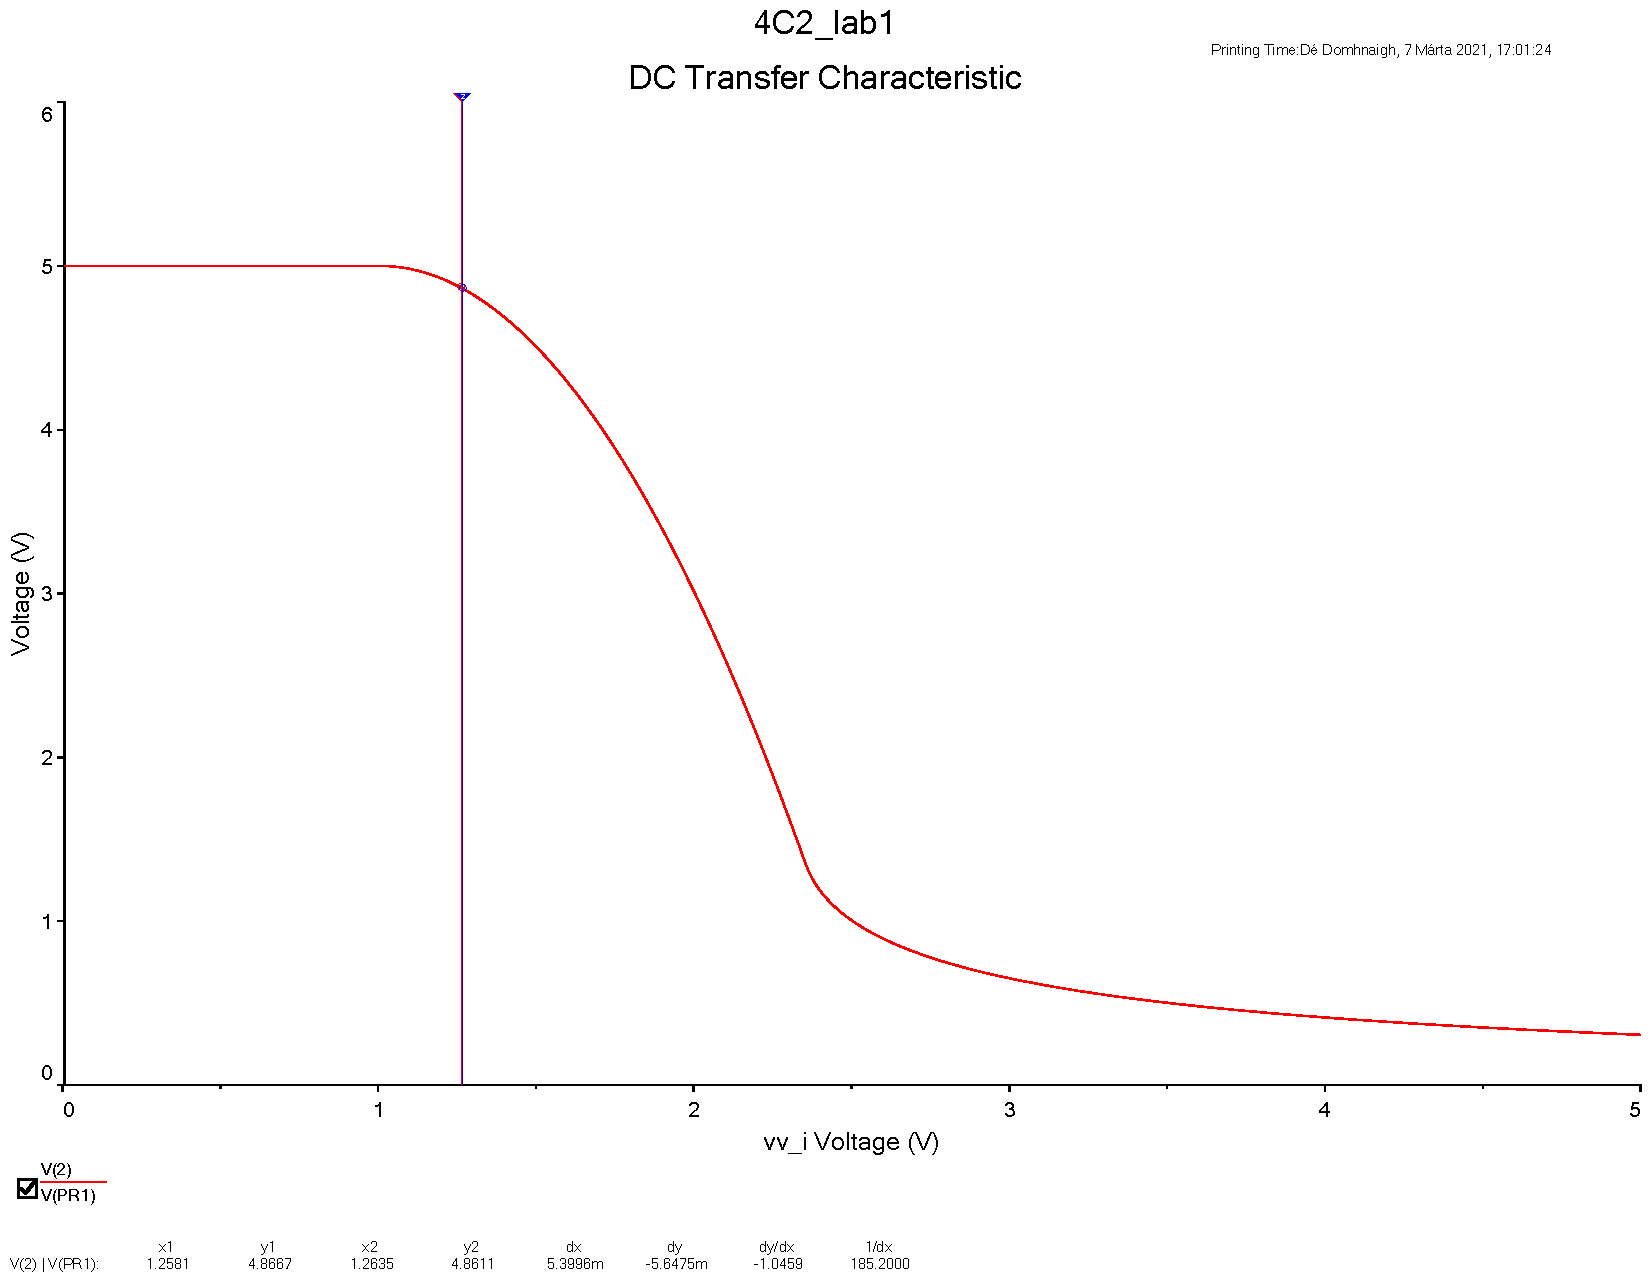
\includegraphics[width=\textwidth]{question_3/100k_ohm_voh_vil} % first figure itself      
  \end{minipage}\vfill
  \begin{minipage}{0.7\textwidth}
      \centering
      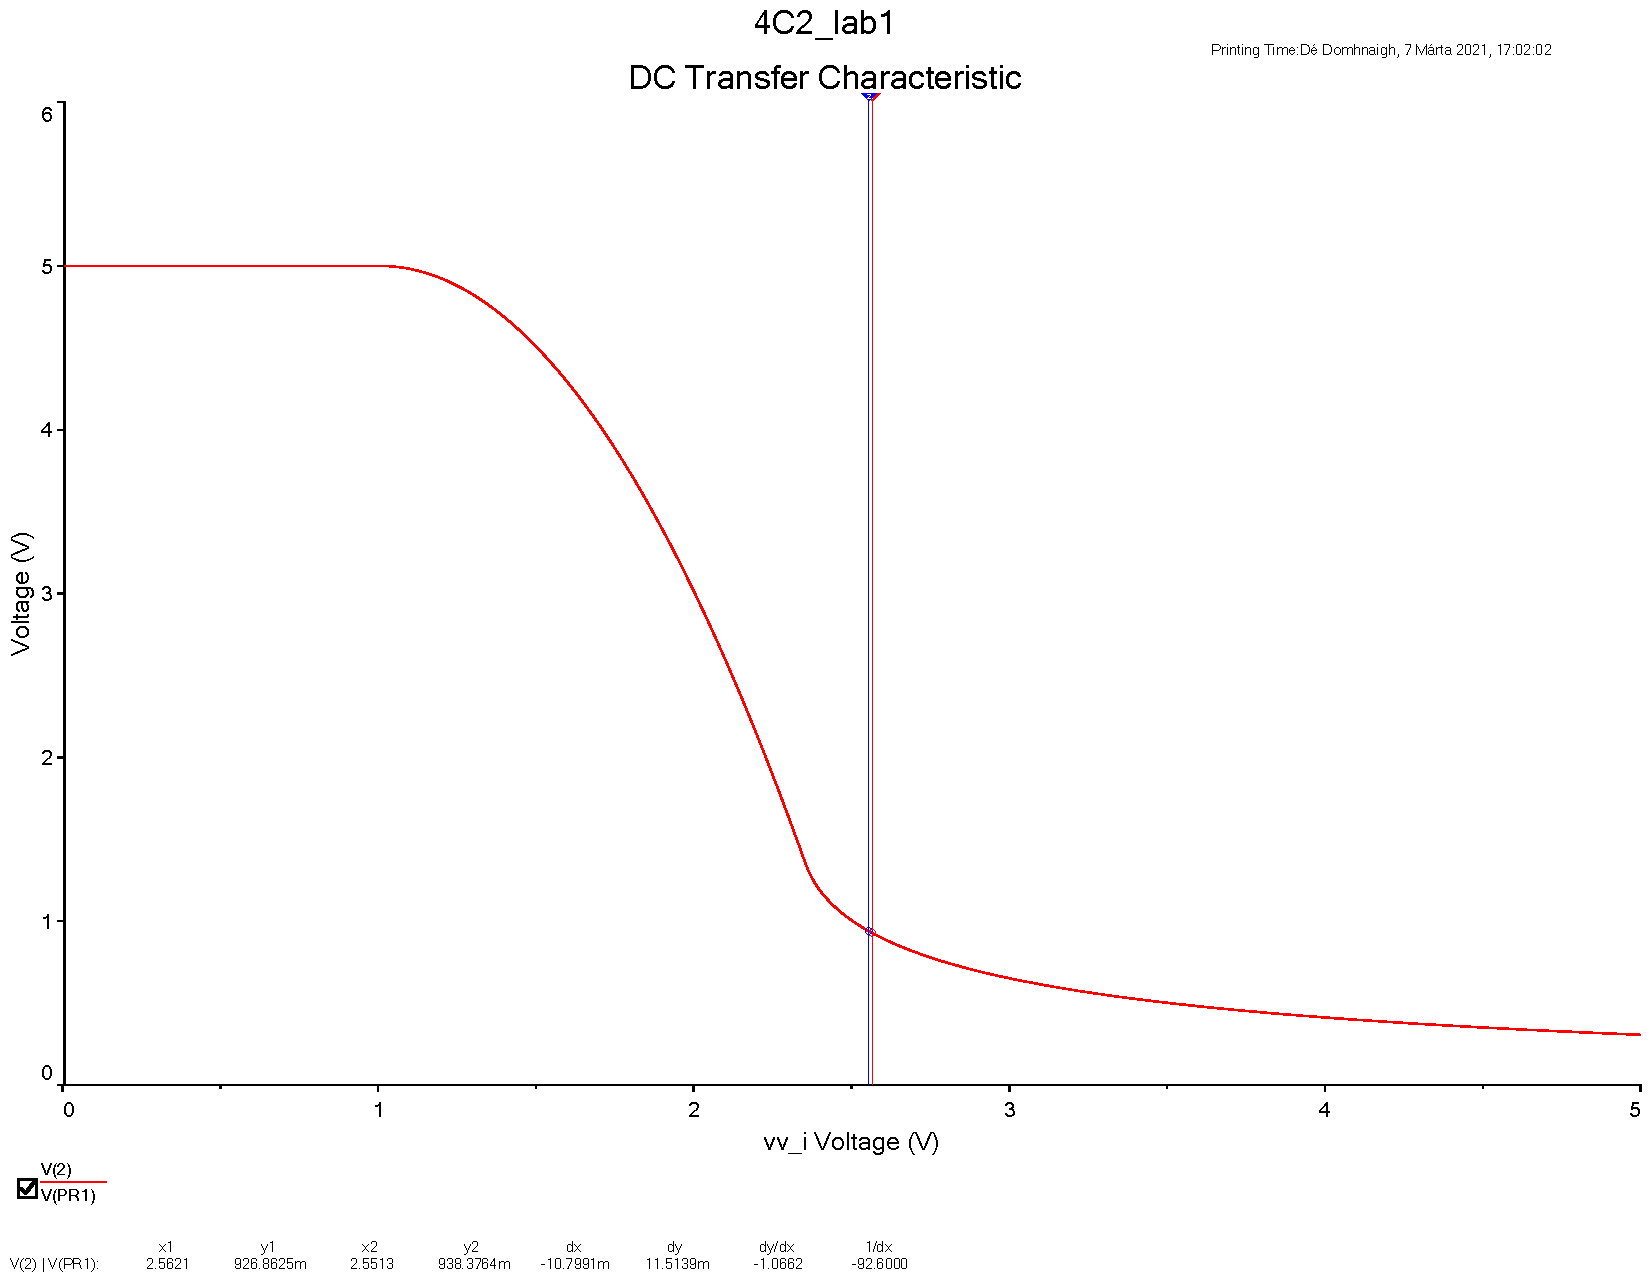
\includegraphics[width=\textwidth]{question_3/100k_ohm_vol_vih} % second figure itself      
  \end{minipage}
  \caption{\centering Plots showing $V_{OH} = 4.877V$ and $V_{IL} = 1.24V$ (top), and $V_{OL} = 0.92V$ and
   $V_{IH} = 2.56$ (bottom), for $R = 100k\Omega$}  
   \label{fig:10}
\end{figure}

From figure \ref{fig:10} we can see the values $V_{OH} = 4.877V$, $V_{IL} = 1.24V$, $V_{OL} = 0.92V$, 
$V_{IH} = 2.56$ closely match the expected values of these quantities which have been calculated in equations \ref{eq:2.2.2.1}, to \ref{eq:2.2.2.4}.

\begin{gather}
  V_{OH} = 5 - \frac{1}{2} \times \frac{1}{4} = 4.875V\label{eq:2.2.2.1}\\
  V_{IL} = 1 + \frac{1}{4} = 1.25V\label{eq:2.2.2.2}\\
  V_{OL} = \sqrt{\frac{2}{3} \times 5 \times \frac{1}{4}} = 0.91V \label{eq:2.2.2.3}\\
  V_{IH} = 1 + \sqrt{\frac{8}{3} \times 5 \times \frac{1}{4}} - \frac{1}{4} = 2.576V\label{eq:2.2.2.4}
\end{gather}



\newpage
\section{Propagation Delay of an RC Circuit}
\FloatBarrier


\begin{figure}[h]
    \centering
    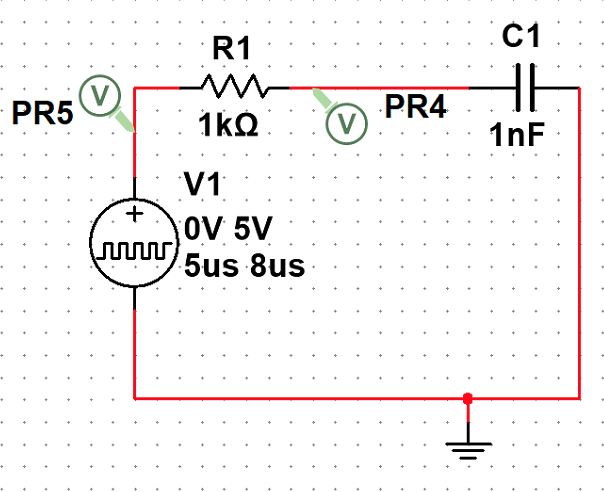
\includegraphics[width=0.45\textwidth, trim={0 0cm  0 0},clip]{report/img/question_4/circuit4.png}
    \captionsetup{justification=centering}
    \caption{Circuit constructed to measure the transient response of capacitor C1.}
    \label{fig:circuitq4}
\end{figure}


The circuit in figure \ref{fig:circuitq4} was constructed to analyse the transient response of the RC circuit.



\begin{figure}
  \centering
  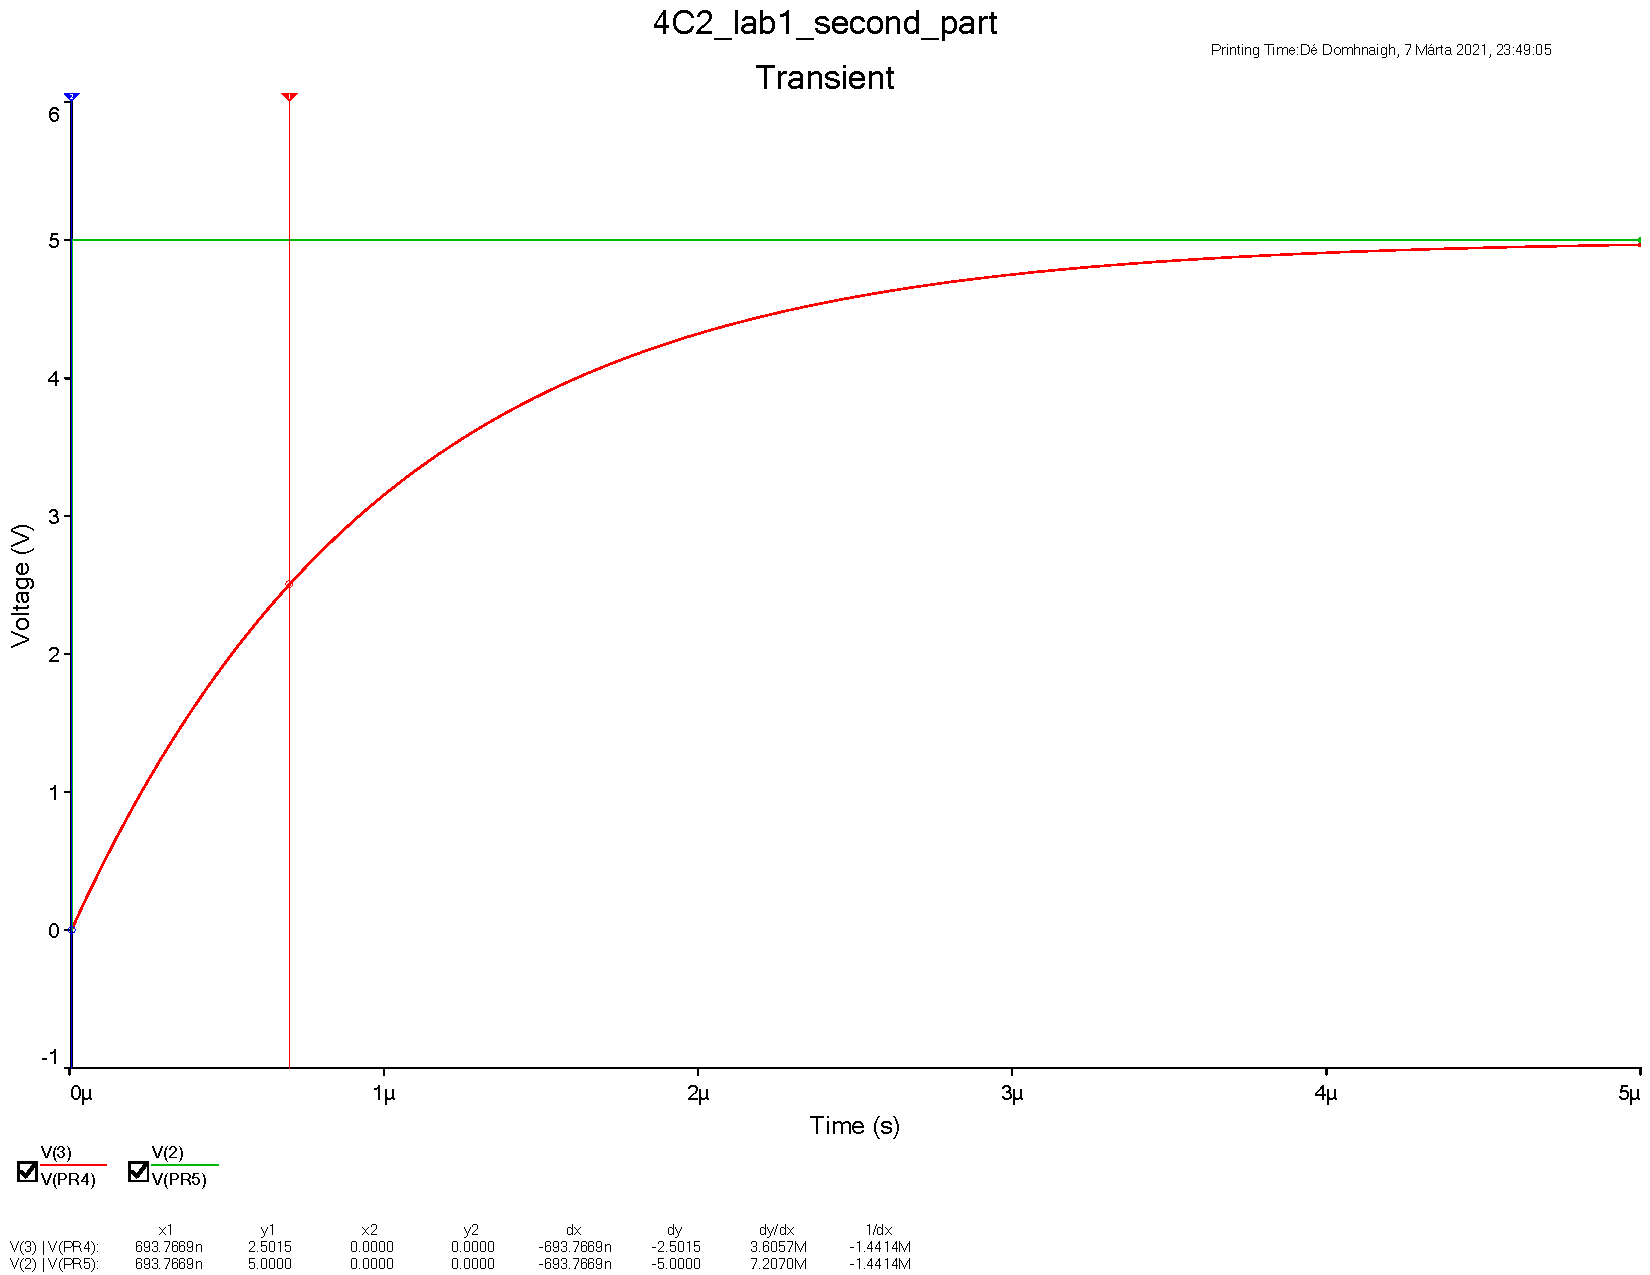
\includegraphics[width=\textwidth]{report/img/question_4/rise_time_0u.pdf}
  \caption{\centering Output graph of $V_i$ and $V_O$ with a $0\mu$ rise time, showing a propagation delay of $t_p = 0.694 \mu s$.}
    \label{fig:0rt}
\end{figure}

From the transient analysis of the circuit, it can be seen in figure \ref{fig:0rt} that the propagation delay of the circuit is $t_p = 0.694 \mu s$. This result is to be expected and can be verified using the following method:

\begin{enumerate}
    \item Consider the circuit in figure \ref{fig:circuitq4} in the Laplace domain. In the Laplace domain the resistor will still have a value R, however the capacitor will now have a value of $\frac{1}{sC}$.
    \item Use the voltage divider rule to form an expression for $V_o$:
        \begin{equation}
            \label{eq:circ}
            V_o(s) = V_i(s) \times \frac{\frac{1}{sC}}{sC + R}
        \end{equation}
    \item The behaviour of the input voltage can be treated as a step function, which in the Laplace domain will be represented by the expression:
    \begin{equation}
        \label{eq:us}
        \frac{V_{DD}}{s}
    \end{equation}
    \item Combining equation \ref{eq:circ} and \ref{eq:us} and rearranging produces the following expression:
    \begin{equation}
        V_o(s) = \frac{V_{DD}}{RC} \times \frac{1}{s\big(s + \frac{1}{RC}\big)}
    \end{equation}
    
    \item Applying the inverse Laplace transform we are left with equation 
    \begin{equation}
        V_{o}(t) = V_{DD} \big( 1 - e^{- \frac{t_p}{RC}} \big)
    \end{equation}
    
    \item To find the propagation delay for $V_o$ to reach 50\% of it's final value, substitute in the $0.5V_{DD}$ for $V_{o}(t)$ and solve for $t_p$:
    \begin{gather}
        0.5V_{DD} = V_{DD} \big( 1 - e^{- \frac{t_p}{RC}} \big)   \\
        t_p = 0.693RC
    \end{gather}
    \item When using the values for R and C from circuit \ref{fig:circuitq4}, $R = 1K\Omega$ and $C = 1nF$, we will get $t_p = 0.693 \mu s$ which corresponds to the value observed from the simulation of the circuit in figure \ref{fig:0rt}.
\end{enumerate}

\subsection{Increasing the rise time}
Increasing the rise time of $V_i$ results in an increase in the propagation delay $t_p$ as can be seen in figures \ref{fig:2rt} - \ref{fig:1rt}, where the rise time of $V_i$ is increased from $0.2 \mu s$  to
$1\mu s$ and the propagation delay increases from $0.697\mu s$ to $0.734\mu s$ as a result. As the rise time is increased the propagation delay deviates further from the time constant, RC.

The impact that the rise time has on the propagation delay can be experimentally modeled using the following equation:
\begin{equation}
    t_p = k \tau
\end{equation}
Where $\tau$ is the RC time constant $\tau = 0.693RC$.

\begin{table}[h!]
\centering
\caption{\centering Increasing the rise time of $V_i$ causes in an increase in the propagation delay $t_p$.}
\label{tab:pd}
    \begin{tabular}{c|c|c}
         Rise Time ($\mu s$) & $k$ & Propagation Delay $t_p$ ($\mu s$)\\
         \hline
         $0$ & $1$ & $0.693$ \\
         $0.2$ & $1.004$ & $0.697$ \\
         $0.4$ & $1.007$ & $0.699$ \\
         $0.6$ & $1.019$ & $0.707$ \\
         $0.8$ & $1.039$ & $0.721$ \\
         $1$ & $1.058$ & $0.734$ \\
    \end{tabular}
\end{table}

\begin{figure}[h!]
  \centering
  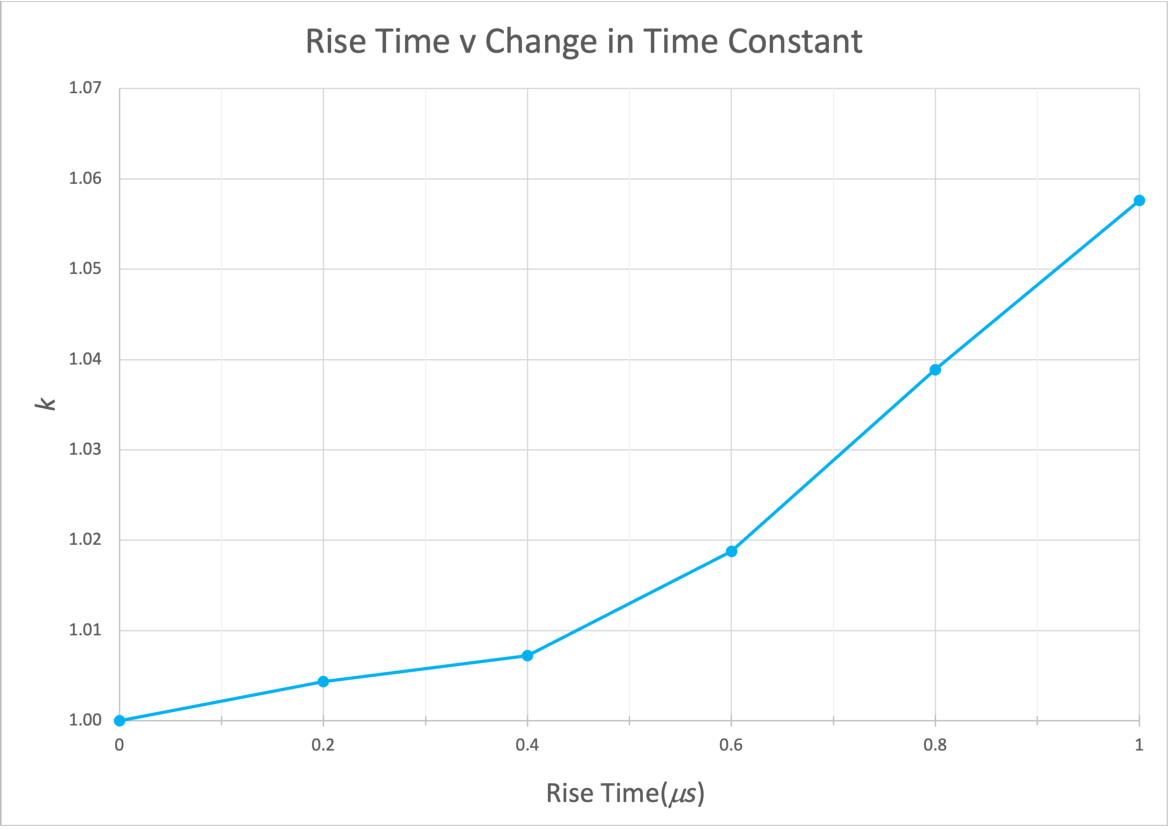
\includegraphics[width=\textwidth]{report/img/question_4/rise_time_time_constant.pdf}
  \caption{\centering Graph of the change in the time constant $t_p$ as a result of the change in the rise time of the input signal $V_i$.}
    \label{fig:2rt}
\end{figure}

\begin{figure}[h!]
  \centering
  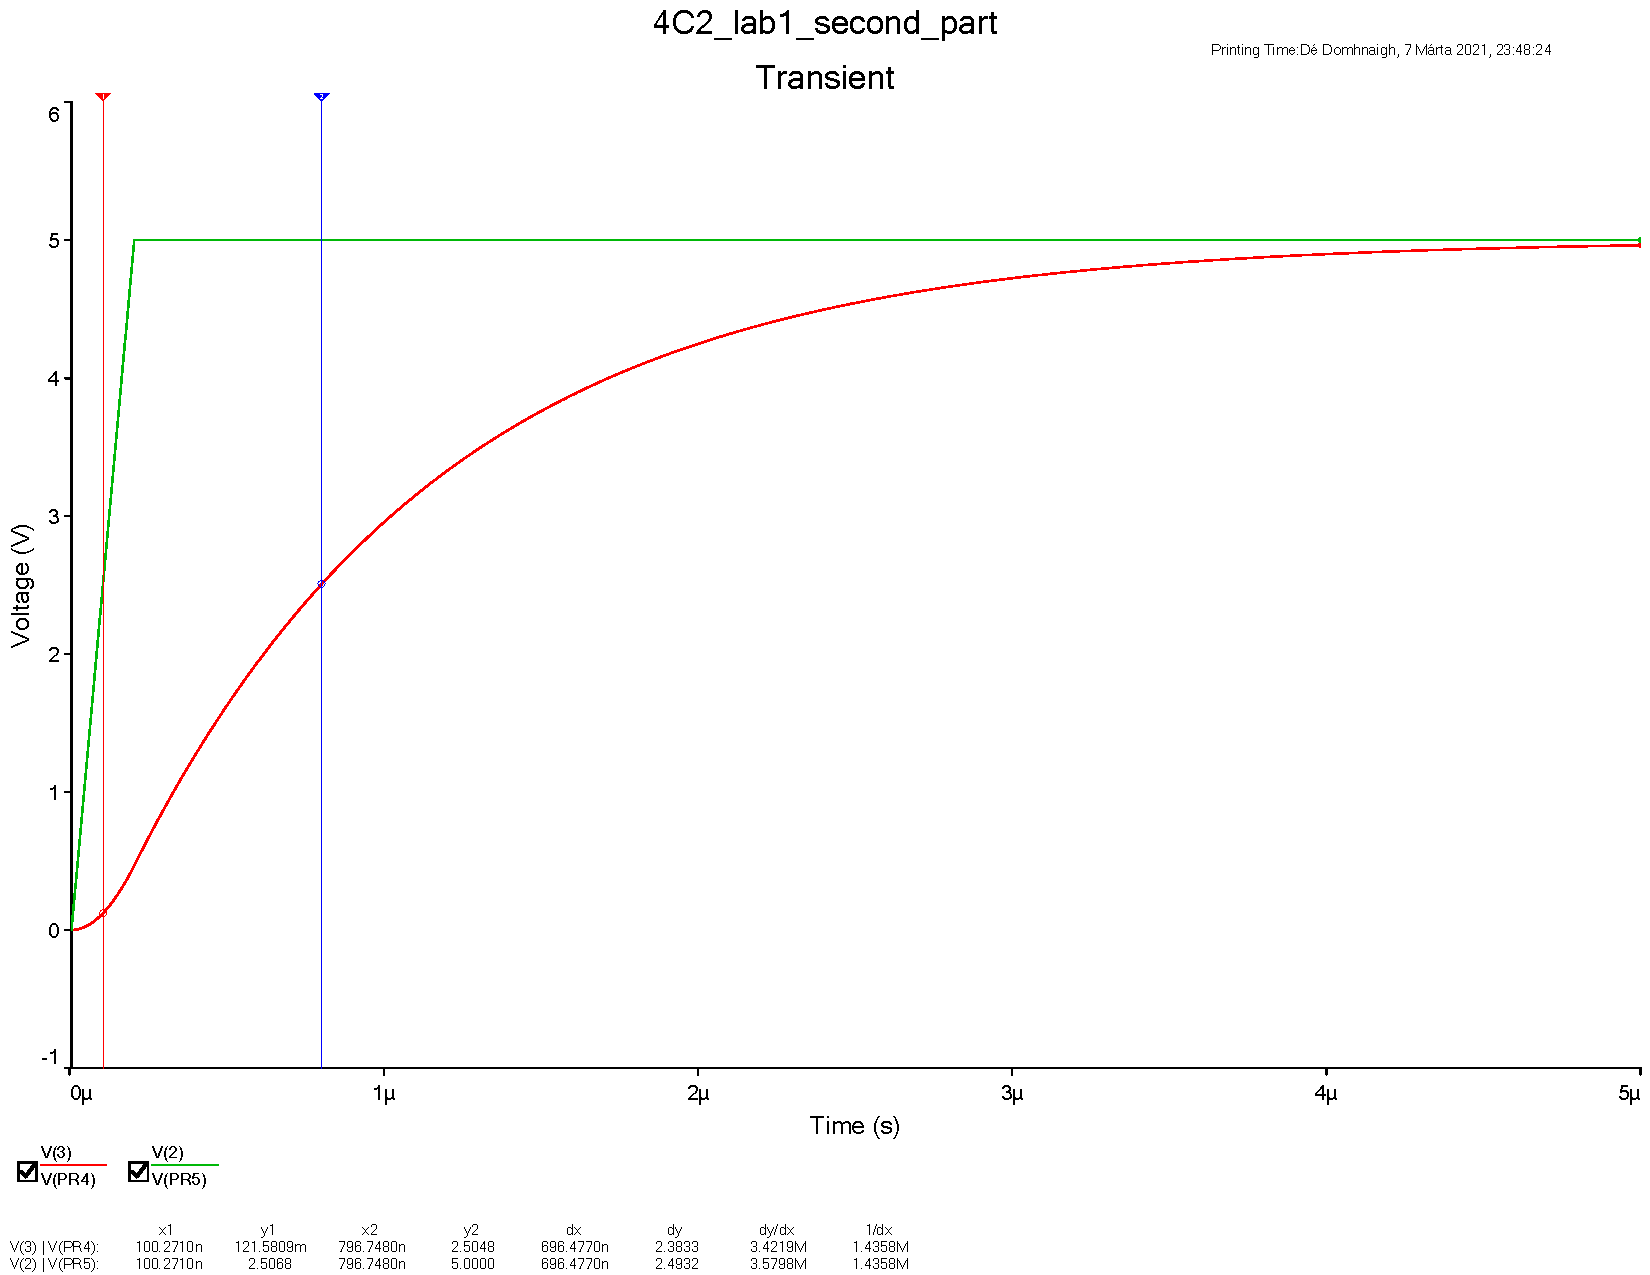
\includegraphics[width=0.9\textwidth]{report/img/question_4/rise_time_02u.pdf}
  \caption{\centering Output graph of $V_i$ and $V_O$, for circuit 4, with a $0.2\mu$ rise time, showing a propagation delay of $t_p = 0.697 \mu s$.}
    \label{fig:2rt}
\end{figure}

\begin{figure}
  \centering
  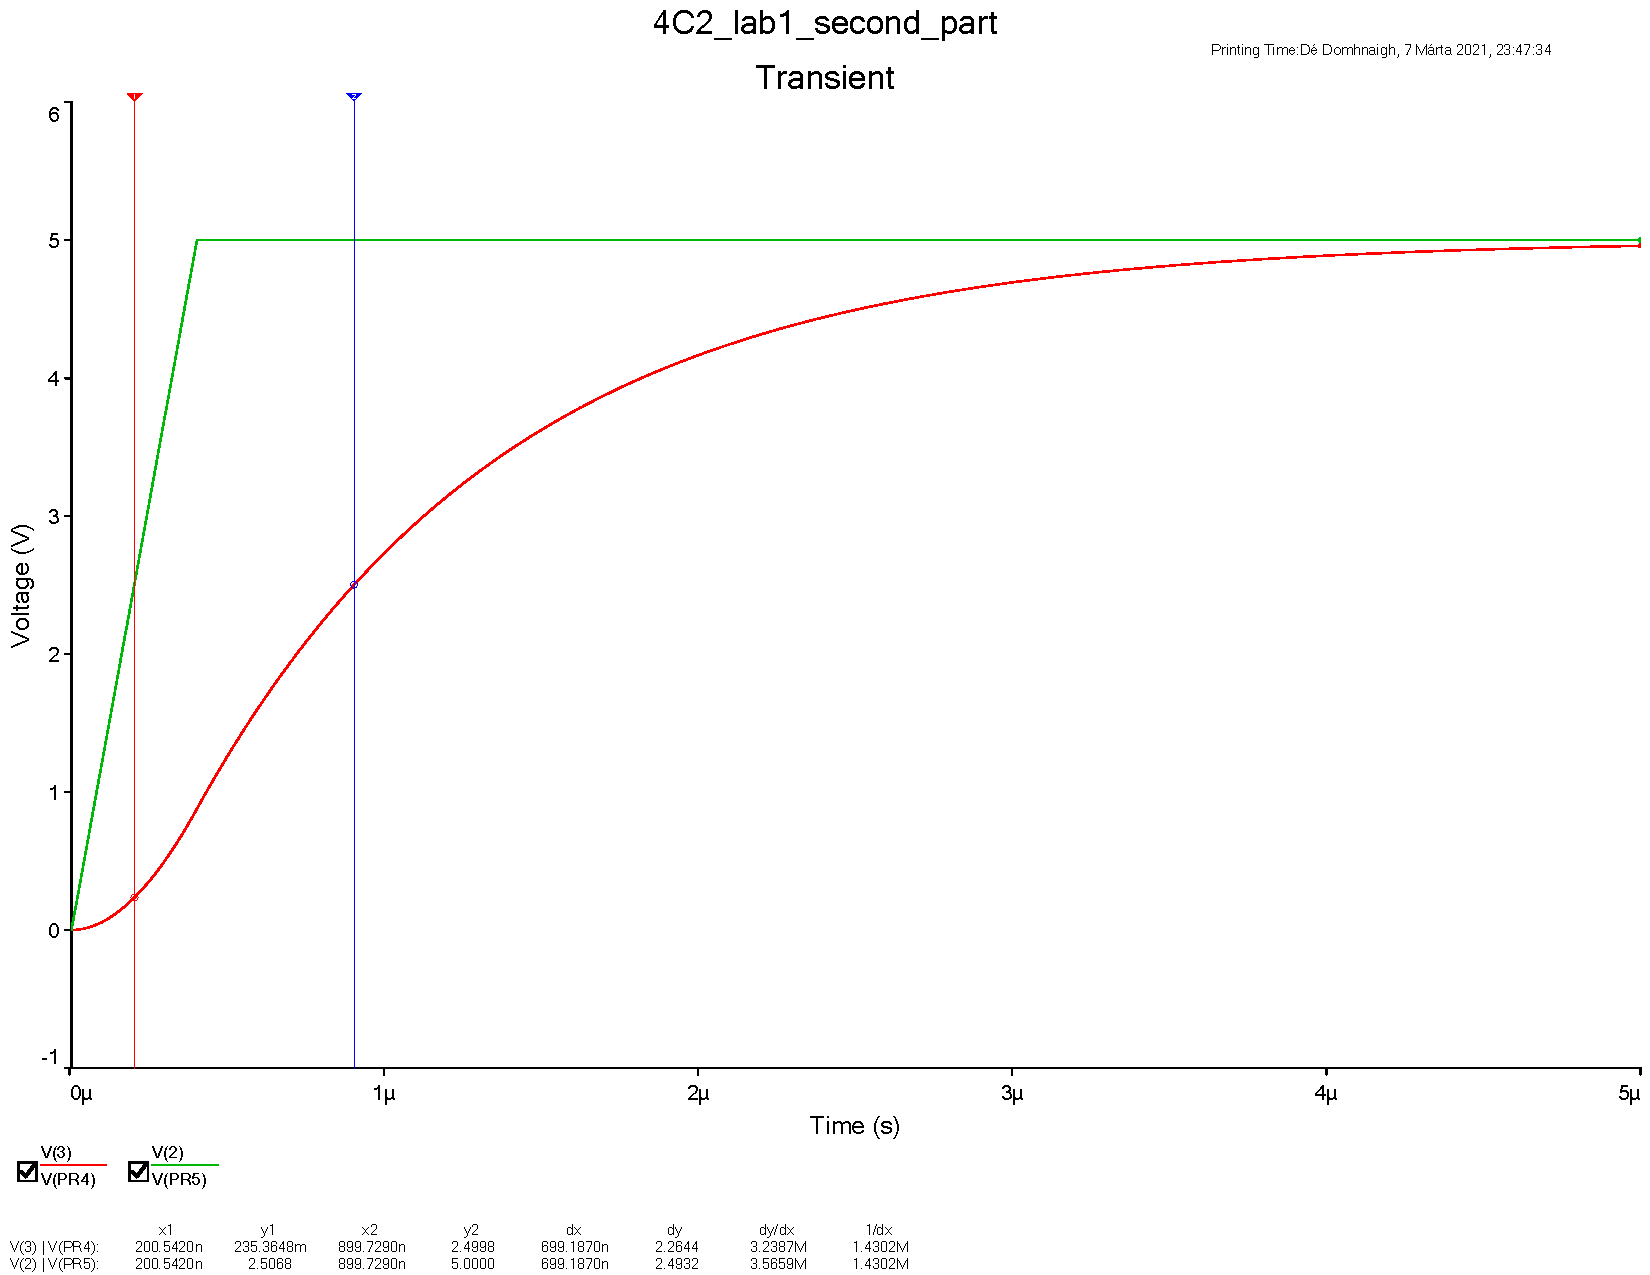
\includegraphics[width=\textwidth]{report/img/question_4/rise_time_04u.pdf}
  \caption{\centering Output graph of $V_i$ and $V_O$, for circuit 4, with a $0.4\mu$ rise time, showing a propagation delay of $t_p = 0.699 \mu s$.}
    \label{fig:4rt}
\end{figure}

\begin{figure}
  \centering
  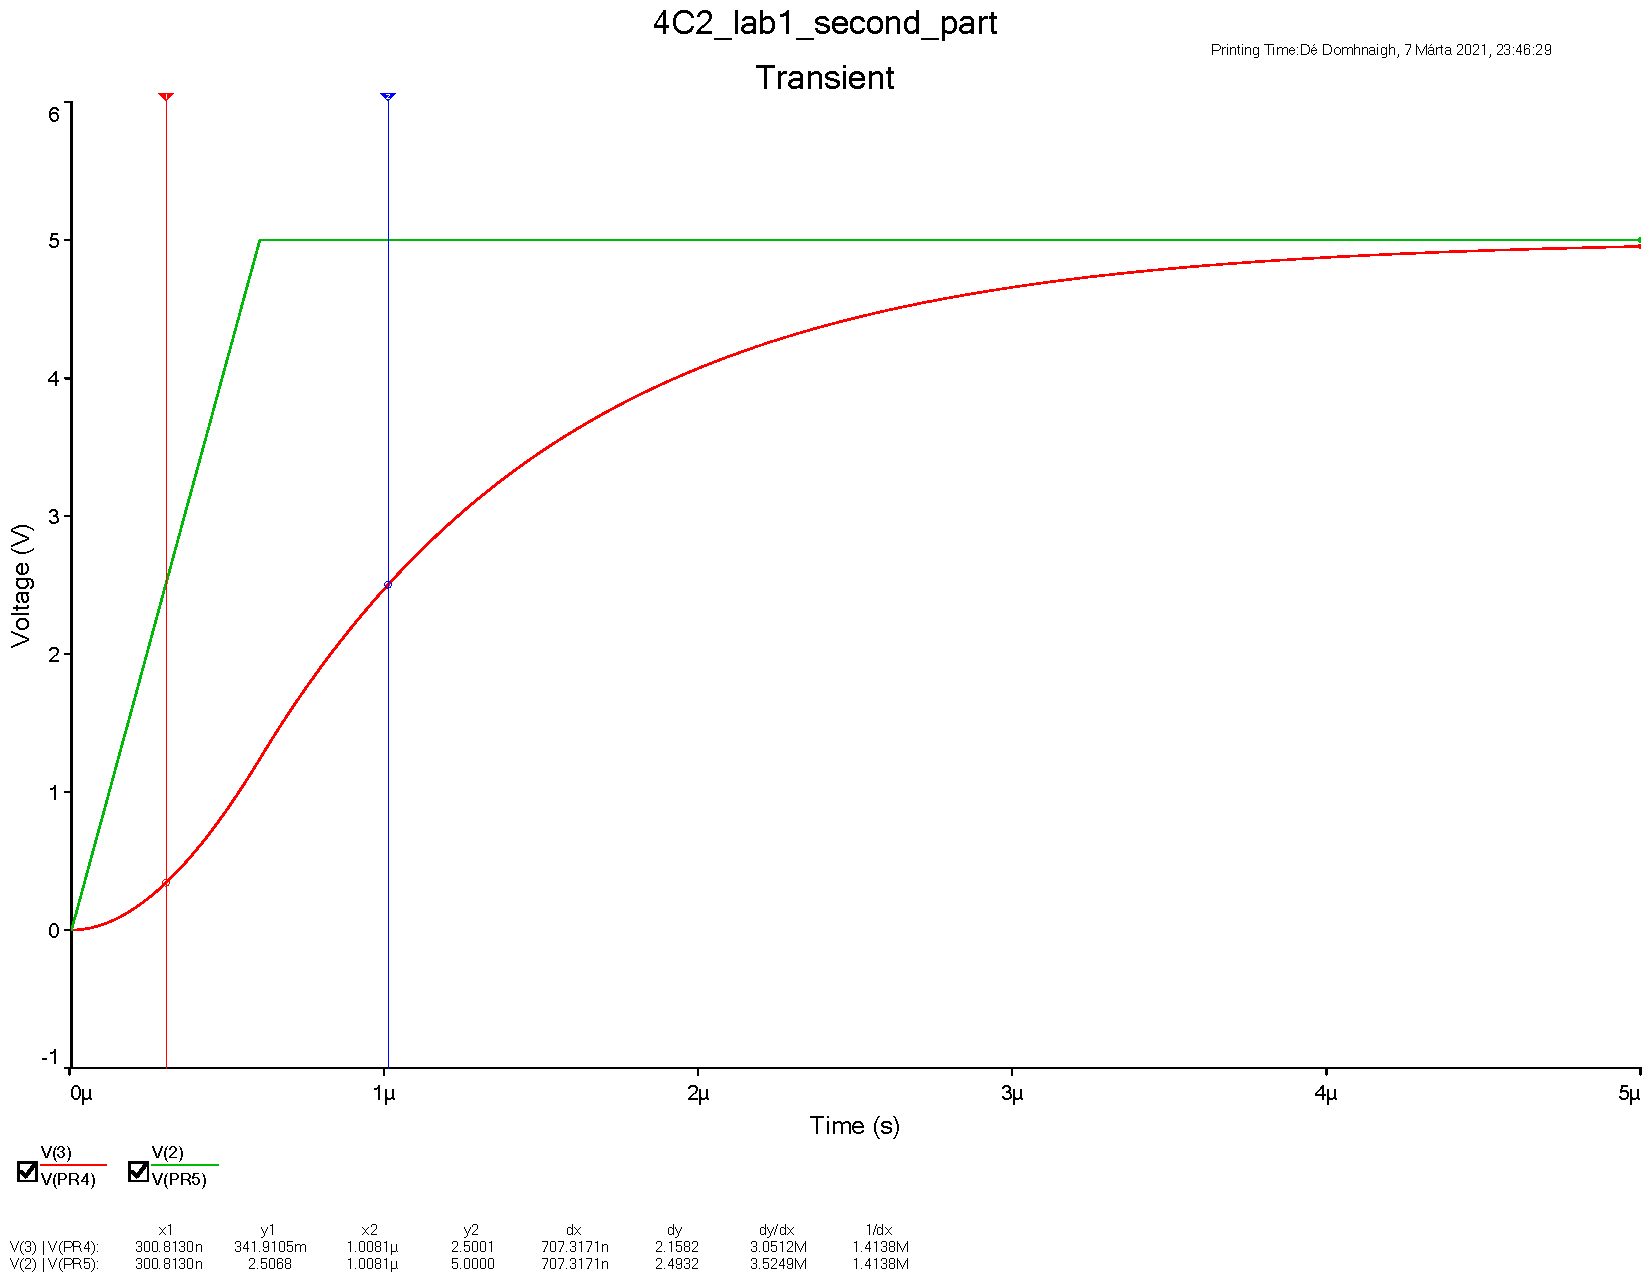
\includegraphics[width=\textwidth]{report/img/question_4/rise_time_06u.pdf}
  \caption{\centering Output graph of $V_i$ and $V_O$, for circuit 4, with a $0.6\mu$ rise time, showing a propagation delay of $t_p = 0.707 \mu s$.}
    \label{fig:6rt}
\end{figure}

\begin{figure}
  \centering
  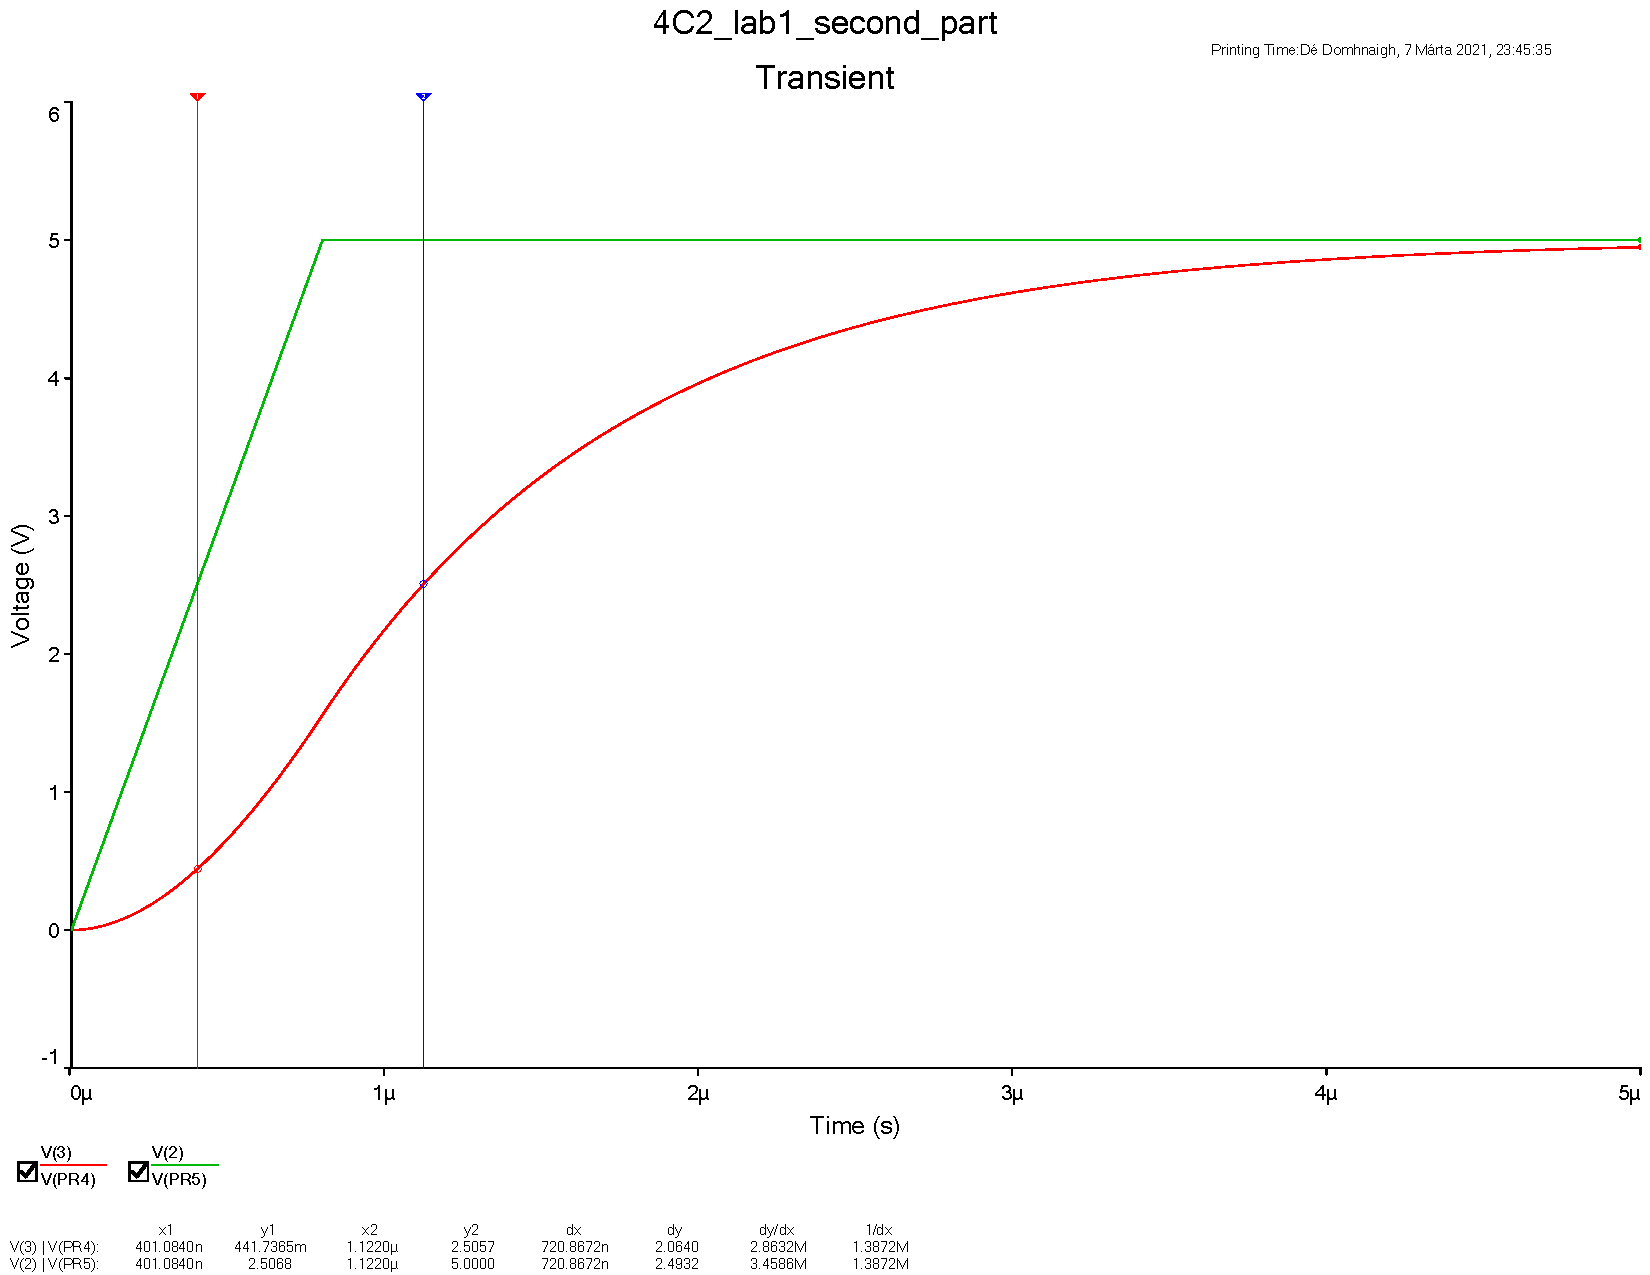
\includegraphics[width=\textwidth]{report/img/question_4/rise_time_08u.pdf}
  \caption{\centering Output graph of $V_i$ and $V_O$, for circuit 4, with a $0.8\mu$ rise time, showing a propagation delay of $t_p = 0.721 \mu s$.}
    \label{fig:8rt}
\end{figure}


\begin{figure}
  \centering
  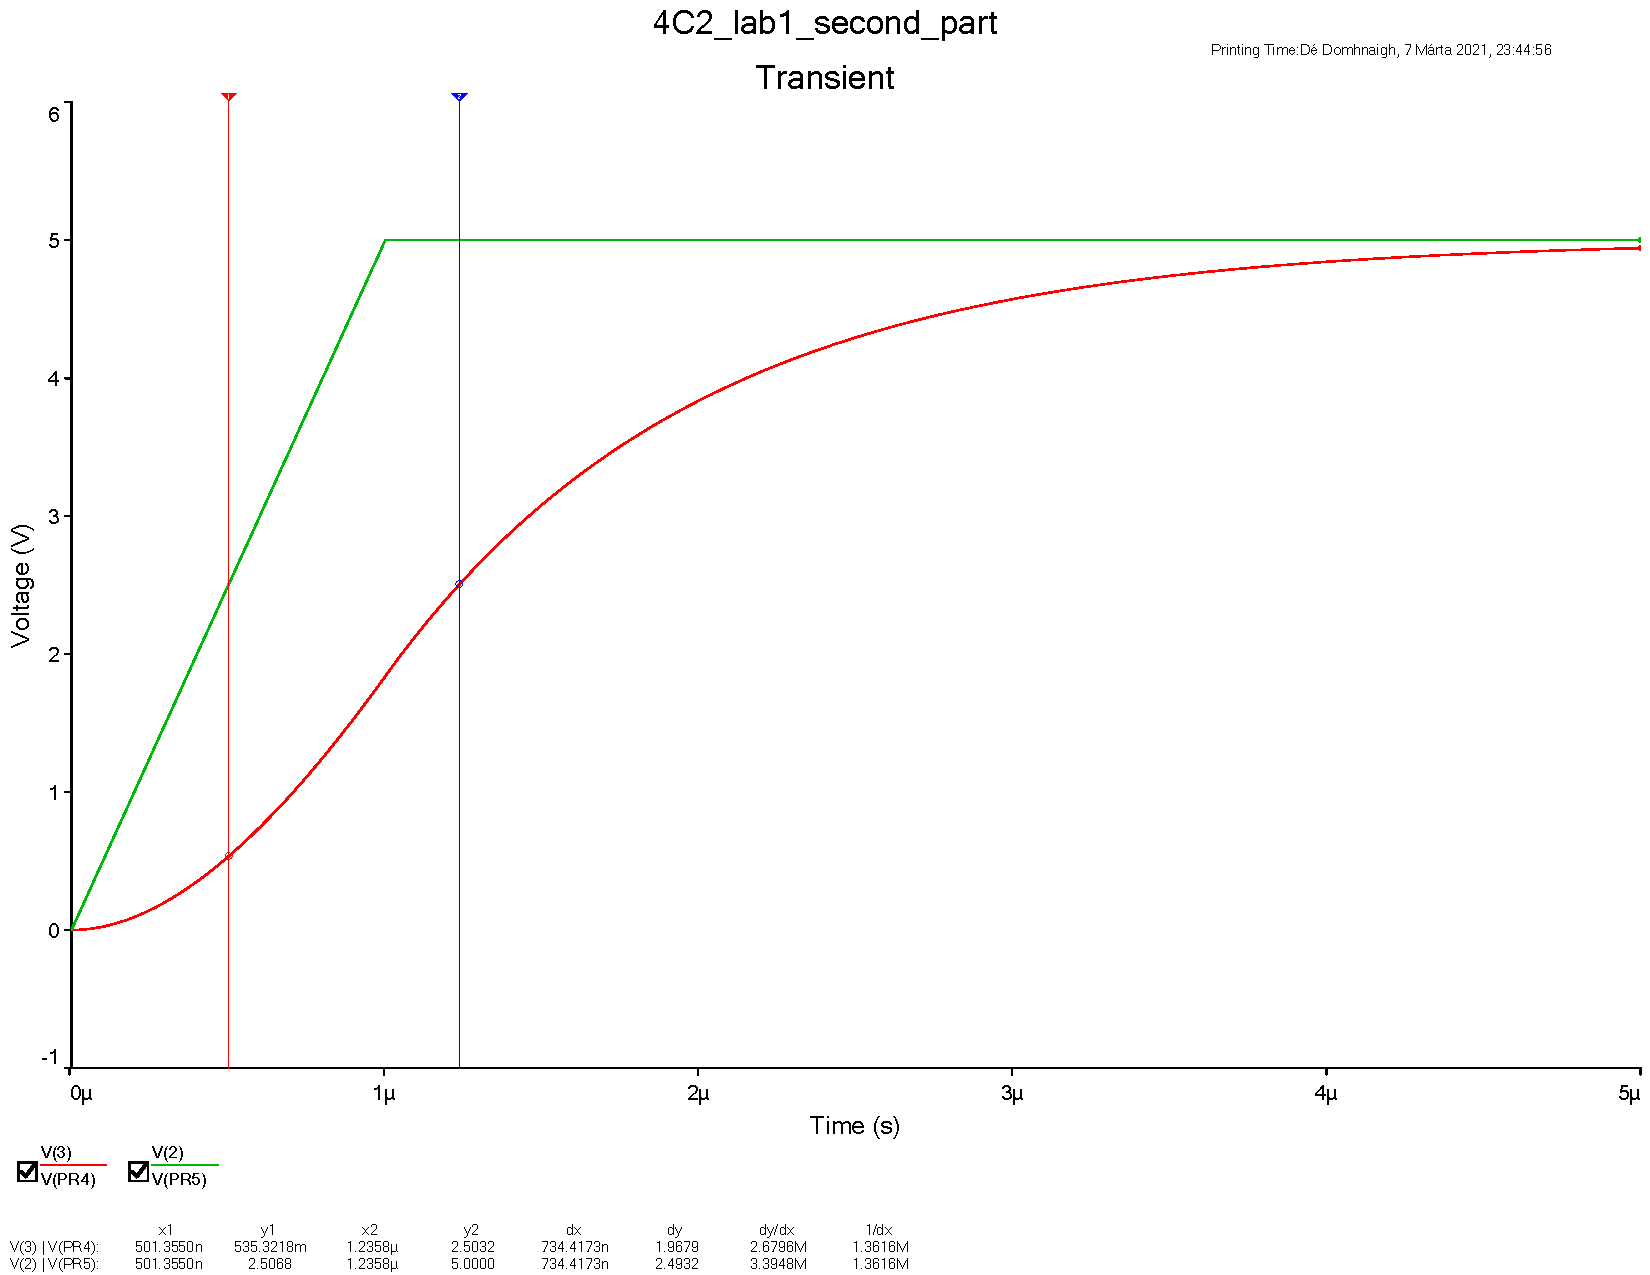
\includegraphics[width=\textwidth]{report/img/question_4/rise_time_1u.pdf}
  \caption{\centering Output graph of $V_i$ and $V_O$, for circuit 4, with a $1\mu$ rise time, showing a propagation delay of $t_p = 0.734 \mu s$.}
    \label{fig:1rt}
\end{figure}


\end{document}
 